\documentclass{article}
\usepackage[english]{babel}
\usepackage[english]{isodate}
\usepackage[style=ieee,backend=bibtex,defernumbers=true]{biblatex}
\addbibresource{9_references-scholar.bib}
\addbibresource{9_references-other.bib}

\usepackage{amsmath}
\usepackage[margin=1in]{geometry}
\usepackage{hyperref}
\usepackage{booktabs}
\usepackage{multirow}
\usepackage{tikz}
\usepackage{pgfplots}
\usepackage{standalone}
\usepackage{xcolor}
\usepackage{standalone}
\usepackage{tabularx}
\usepackage{subfig}
\usepackage{csquotes}
\usepackage{float}
\usepackage{xcolor}
\usepackage{listings}
\usepackage{adjustbox}
\usepackage{subfig}
\usepackage{multicol}
\usepackage{algorithm}
\usepackage[noend]{algpseudocode}
\usepackage{listings}
\usepackage{xcolor}
\usepackage[utf8]{inputenc}
\usepackage[defaultlines=5,all]{nowidow}
\usepackage{fancyhdr}
\usepackage{changepage}

\pagestyle{fancy}
\fancyhf{}
\rhead{Detecting Road Surface Anomalies using Multimodal Machine Learning}
\lhead{Joël Luijmes, 2021}
\cfoot{\thepage}

\definecolor{codegreen}{rgb}{0,0.6,0}
\definecolor{codegray}{rgb}{0.5,0.5,0.5}
\definecolor{codepurple}{rgb}{0.58,0,0.82}
\definecolor{backcolour}{rgb}{0.95,0.95,0.92}

\lstdefinestyle{mystyle}{
    backgroundcolor=\color{backcolour},   
    commentstyle=\color{codegreen},
    keywordstyle=\color{magenta},
    numberstyle=\small\color{codegray},
    stringstyle=\color{codepurple},
    basicstyle=\ttfamily,
    breakatwhitespace=false,         
    breaklines=true,                 
    captionpos=b,                    
    keepspaces=true,                 
    numbers=left,                    
    numbersep=5pt,                  
    showspaces=false,                
    showstringspaces=false,
    showtabs=false,                  
    tabsize=2,
    escapeinside={``}
}

\lstset{style=mystyle}


\definecolor{light-gray}{gray}{0.95}
\definecolor{darkblue}{rgb}{0, 0, 0.5}
\hypersetup{colorlinks=true,citecolor=darkblue, linkcolor=darkblue, urlcolor=darkblue}

% \widowpenalties 1 10000
% \raggedbottom

\usepackage{charter}
\usepackage[parfill]{parskip}

\usepackage{enumitem}
\setlist[itemize,enumerate]{noitemsep, topsep=0.5pt}

% \bibliographystyle{IEEEtranN}

\newcommand{\authorref}[1]{\citeauthor*{#1} (\citeyear{#1}) \cite{#1}}
\newcommand{\code}[1]{%
\setlength\fboxsep{1pt}%
\colorbox{backcolour}{\lstinline{#1}}%
}


\setcounter{tocdepth}{2}

\begin{document}

\pagenumbering{arabic}

\title{
    \textbf{Detecting Road Surface Anomalies using\\
    Multimodal Machine Learning}
}
\author{
\textbf{Joël Luijmes} \\ 
\small{Student number: 2031107} \\
\small{Email: \href{mailto:me@joell.app}{me@joell.app}}
}

\date{}
\maketitle
\thispagestyle{empty}

\vskip 3cm

{\centering

THESIS SUBMITTED IN PARTIAL FULFILLMENT \\
OF THE REQUIREMENTS FOR THE DEGREE OF \\
MASTER OF SCIENCE IN DATA SCIENCE AND ENTREPRENEURSHIP \\
JHERONIMUS ACADEMY OF DATA SCIENCE

\vskip 6cm

Supervisors: \\
Prof. Dr. Willem-Jan van den Heuvel \\
Dr. Dario Di Nucci

\vskip 3cm

Jheronimus Academy of Data Science \\
1 December 2021

\par}

\newpage
\thispagestyle{empty}
\mbox{}
\newpage
\thispagestyle{empty}

\section*{Abstract}

\begin{adjustwidth}{1cm}{2cm}
\textit{The current process of performing road maintenance takes long, is costly and largely relies on subjective observations. In recent years, the need for data driven inspection emerged to perform automatic road quality assessment. In this work, we contribute a novel method combining both visual and accelerometer data to detect road surface anomalies. We evaluate the performance of the multimodal model with that of respective unimodal models. The visual based model performs best with an precision of 0.86, followed by the hybrid fusion model with precision of 0.66. Our results indicate that multimodal machine learning is successful in detecting manholes.
}
\end{adjustwidth}


\newpage
\thispagestyle{empty}
\mbox{}
\newpage
\thispagestyle{empty}

\tableofcontents

\clearpage
\section{Introduction}

In the Netherlands, public infrastructure maintainers (the state, provinces, municipalities and water authorities) have the legal responsibility for maintaining their assets. Maintaining the road means "to ensure that all roads within the area are in good condition" \cite{Wegenwet} . In this sense road maintainers are obliged to maintain facilities regularly and sustainable \cite{BurgerlijkWetbook6:174}. In order to give some guidance on how to assess the state of roads, standards are made by the national knowledge platform CROW. Among it activities the CROW prescribes road maintainers how to perform and assess road inspections \cite{CROW_147}. CROW helps maintainers in quality-driven management. 

Road maintenance is a big expenditure of the state's budget, it is annually around 2.5 - 3.5 billion (x1.000.000.000) EUR \cite{Rijksbegroting:Infrastructuur}. Depending on the type of the road, a different public body is responsible for maintaining that road. For instance, highways (indicated with A) are maintained by the state (Rijkswaterstaat), provincial (indicated with N) roads by the provinces, and local roads (indicated with street names) by municipalities. Public bodies are legally obliged to report "maintenance capital goods" in their annual budgets \cite{Wet_Besluit_Begroting}. Within the report they have to state the policy framework for maintenance and the financial implications. From this, it flows that road maintenance is planned through a multi-year plan. Programming for multi-year road maintenance requires clear insights in current road conditions. Road maintenance is a significant expensive, and being public money, it is important that it is well spent. 

\begin{figure}[ht]
    \begin{center}
    \includegraphics[height=6cm]{images/1_introduction/budget.png}
    \end{center}
    \caption{Budget for maintenance of public roads \cite{Rijksbegroting:Infrastructuur}. Budget is in billion (x1.000.000.000) EUR.}
    \label{fig:prm}
\end{figure}

Road maintenance is performed according to an annual cyclical process. The road owner or maintainer (i.e. state, province or municipality) initiates a tender for inspection. After which, an inspection company inspects the road with specialized vehicles. This vehicle contains of multiple cameras to record the road surface, infrared sensor to measure the evenness, and other types of sensors. The recorded video data is manually inspected by engineers according the prescribed CROW method \cite{CROW_147}. The inspection company delivers a report with recommendations to the road owner indicating which roads needs maintenance. On this recommendation, the road owner initiates another tender to perform the actual maintenance. Interestingly to note is that companies that can perform inspections, often also can perform the construction.

The condition of the road can thus measured through various quantifiable data sources. Below is a list given of data sources which are often used within the Netherlands for road inspection:
\begin{itemize}
\item Visual inspection: video data is manually annotated to mark damages.
\item ARAN measurements: laser sensor which measures distance between the road and vehicle across the pavement. This can be used to measure the surface unevenness or rutting.
\end{itemize}
\begin{itemize}
\item Ground penetrating radar: geophysical method which uses radar pulses to get an image of the subsurface by measuring the reflected signals. This enables to assess the quality of the asphalt and deeper layers, detect sinkholes and can detect objects below the surface.
\item Falling weight deflector: similar to ground penetrating radar, but instead of using radar pulses, a weight is dropped and reflections are measured. This method is more commonly used in civil engineering. 
\item Skid resistance: describes the force when a locked tire (i.e. a wheel that is prevented from rotating) slides along the surface. Measurements are performed by measuring the friction on the locked wheel. This method is used to detect if the road is too slippery e.g. aquaplaning.
\item Static data:  besides actual measurements, there is also static data available about roads.
\begin{itemize}
\item Materials passport describing the different layers of the road. Contains information when and how the layer was constructed and which material was used.
\item Historical maintenance reports.
\item Future date of maintenance (e.g. multi-year plan). 
\item Road intensity (how many vehicles travel the road).
\end{itemize}
    
\end{itemize}
Keeping track of these various sources of data is cumbersome. From experience it appears that  many road owners try to manage this data manually, that is without any specialized software. However, there are some tools in the industry to support their workflow. These software tools are known as "asset management software" or "management systems" . One of the available tools is Predictive Road Maintenance (PRM), a platform for data driven asset management (see figure \ref{fig:prm}). This tool is developed by AssetWorx \footnote{Pronounced as Asset Works}, this is also the startup where this thesis is written. PRM is created during an incubator program known as 'Startup in Residence' funded by the province Overijssel \cite{Residense2020}. As of now (Jul. 2021), PRM is only used by the province Overijssel, but AssetWorx is in active negotiation with other provinces and municipalities for adoption. The ultimate goal is to create an uniform data platform for road maintainers. The idea is to be a disrupter of the industry by providing data driven insights in road quality, maintenance and planning as an independent organization (i.e. not one of existing engineering firms). 

\begin{figure}[ht]
    \begin{center}
    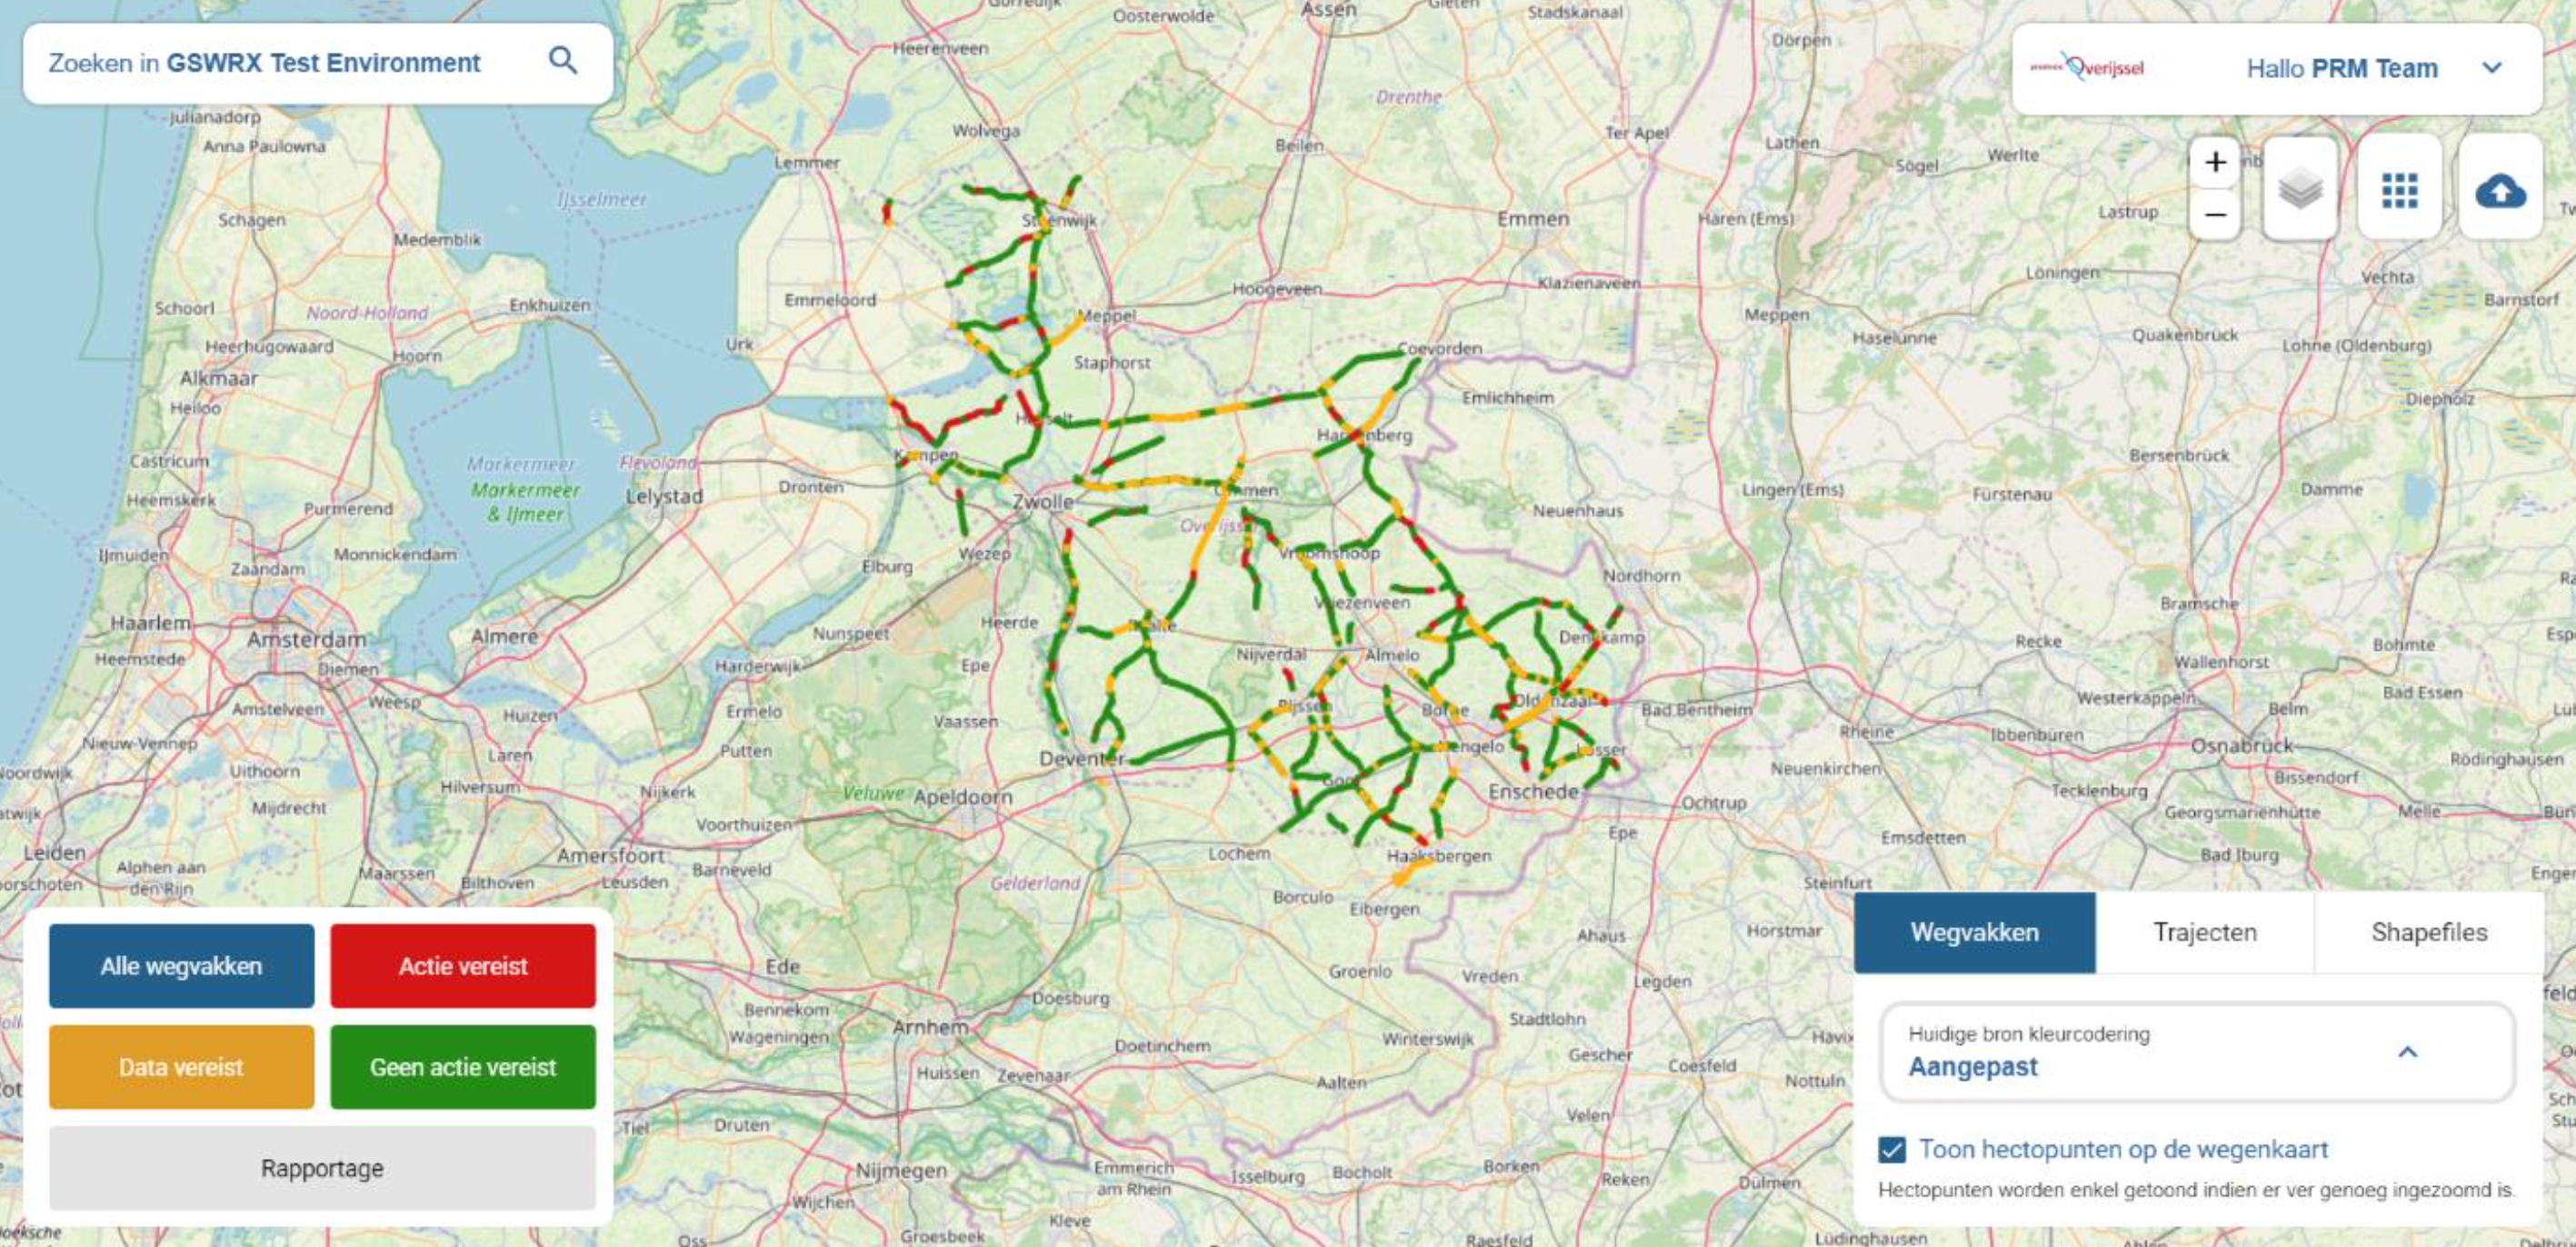
\includegraphics[height=6cm]{images/1_introduction/prm-overview.png}
    \includegraphics[height=6cm]{images/1_introduction/prm-detail.png}
    \end{center}
    \caption{Screenshots of Predictive Road Maintenance (PRM) software.}
    \label{fig:prm}
\end{figure}


\subsection{Relevance}

Although there are other asset management tools in the market, they typically only incorporate one or two data sources. PRM however is designed to operate on all kinds of data, as long the data can be geographically grounded (e.g. GPS coordinates). Currently, almost all road assessment rely on visual inspections based on the CROW systematic \cite{CROW_147}. This is an intensive procedure which largely relies on experience and intuition of the inspectors and maintainers. The cycle of tendering -> inspection -> tendering -> maintenance, typically takes one year. However, when there is a damage in the pavement, the severity of that damage may increase as it remains not repaired. For instance, a pothole starts relatively small but over time, as more traffic passes, it may become a significant damage in the road that eventually affects the drivers. Repairing a small pothole is easy and quick, but as the damages increases, so does the financial costs of repairing a road. Therefore, timely monitoring of road damages saves costs for the maintainer while increasing comfort of driving and safety.

AssetWorx aims to systematically and continuously collect data on roads instead of the conventional annual cycle of inspection and maintenance. Data is manually collected through a sensor box, more details follow in later section. The collected data is then processed to automatically determine the state of the road. In order to determine that state, research (in form of this thesis) is performed to automatically detect road surface damages. None of the existing management tools incorporate this functionality. From online articles, it seems that some construction companies try to pursue this for their own proprietary tools. Automatic detection of road surface defects thus yields a large business value for AssetWorx. When road defects can be detected in a short period, it means that repair costs are minimum, thus yielding a large societal value for road maintainers as well.

Although automatic defect detection have societal and business value, it is scientifically not something new. However, existing literature only utilizes a single source of data (unimodal) to detect damages. For this research, we are collecting various types of data: visual, sound, GPS, accelerations and the CAN bus. The CAN bus is the information bus used connecting different components within a car. Multimodal fusion aims to integrate data of different sources and types in a unified representation \cite{Baltrusaitis2017}. The idea is that by fusion richer information is provided than a single modality can provide. In order to scope the research, we will only be looking at fusing visual and accelerometer data. Within existing literature on road defects detection, multimodal fusion has not been applied. Additionally, fusion of accelerometer and visual data has only been researched in the context of odometry / robot navigation, not to detect damages or objects for that matter. Finally, fusion of visual and accelerometer data is an interesting challenge due time synchronization issue. As the image at timestamp $t_{visual}$ looks ahead, while the accelerometer measures the accelerations at some delay $t_{acc} = t_{visual} + \tau$. 


\subsection{Research Questions}


During this research we are collecting various types of data. To scope our research we only will be looking at fusing visual and accelerometer data. Reason for this is that these sources can be collected in the most reproducible way. The accelerometer is positioned at fixed point inside the vehicle, and a smartphone is attached to the windshield in a conventional holder. Although we also collect sounds and CAN-bus information, these sources are neglected for now. Road noise may not be reliable due conditions (radio, talking), and CAN-bus information differs for each vehicle.

Fusing these visual and accelerometer data is interesting. Visual data can only be recorded in good conditions (i.e. weather and lighting). Complementary, vibrations can always be measured regardless of external conditions. At the same time, interpreting vibration data might pose a difficult task for humans. Combining both data sources helps to interpret the data. With that in mind, this thesis aims to answer the following research question

\begin{itemize}
\item \textbf{RQ: How can we fuse visual and accelerometer data in an end-to-end multimodal deep learning model to classify road surface defects?}
\end{itemize}

In order to answer this question, we can divide it into smaller parts. First of all, to my knowledge, no research has been performed to use multimodal data for detecting road surface defects. However, there have been extensive research on uni-modal data (mostly based on images). To get a better understanding of this field, the first sub question is:

\begin{itemize}
\item \textit{SQ1: What kind of data and algorithms are used to detect road surface defects?}
\end{itemize}

The research is focused on fusing visual and vibration data. In order to fuse these data types, we need to make good representations on each respective data source. The visual data is most easily interpreted by humans. As road surface defects are basically objects in an image, the following research questions is formed:

\begin{itemize}
\item \textit{SQ2: What is state of the art in visual object detection?}
\end{itemize}

Although data fusion hasn't been used in detecting road surface defects, multimodal fusion has been used for visual and accelerometer data.

\begin{itemize}
\item \textit{SQ4: What is the state of the art in combining visual and sensor data for multimodal data fusion?}
\end{itemize}

Specifically we are interested in time synchronization to combine visual and vibration data. Since the camera records front-faced at timestamp $t_{visual}$, the vibration data at $t_{acc}$ is measured with some delay $\tau$. 

\begin{itemize}
\item \textit{SQ5: How to calculate the delay between front-faced visual data and the accelerations of the traveling vehicle?}
\end{itemize}


\subsection{Contributions}

TODO: Write out in actual words / alineas

Contributions of this thesis are as follows:
\begin{itemize}
\item Entrepreneur / social; 
\begin{itemize}
\item Automatic detection of road damages -> saves costs
\item Example data architecture of processing vehicle data on large scale
\end{itemize}
\item Scientific:
\begin{itemize}
\item Novel end-to-end model to detect road surface defects
\item Novel method to fuse future detected object with accelerometer data
\item Open-source code / data?
\end{itemize}
\end{itemize}



\subsection{Remainder}

The remainder of this thesis is structured as follows:

\begin{enumerate}
\addtocounter{enumi}{1}
\item \textbf{Literature} presents the current literature known on the subject. It answers the theoretical research subquestions 1-3. 
\item \textbf{Methodology} explains the methodology that is used during this thesis.
\item \textbf{Data Processing} presents the various data engineering activities required to record and process the data in order to make predictions.
\item \textbf{Multimodal Fusion} deals with the performed experiments.
\item \textbf{Discussion} interprets the results.
\item \textbf{Conclusion} concludes the thesis, and provides some suggestions for future activities.

\end{enumerate}


\clearpage
\section{Related Work}
\label{sec:related-work}

The aim of this section is to describe the existing work that has been done on multimodal machine learning to classify road defects. However, to my knowledge, this has never been researched yet. What we did find is research using a single source of data in machine learning pipelines. This section will therefore review what is known in automatic road defects classification. Finally, we look briefly at current literature on multimodal machine learning in general.

% TODO: table with all keywords and search results

% Literature to answer these questions will be gathered with the following procedure:
% \begin{enumerate}
% \item List search relevant search terms.
% \item Find synonyms in a thesaurus.
% \item Search literature on Google Scholar \cite{scholar}, Science Direct \cite{science-direct} and Papers with Code \cite{paperswithcode}. 
% \item Select potential papers based on their title and abstract.
% \item Check Google Scholar which cite the respective paper to see if a more recent version exists (forward citation).
% \item Scan through paper references if a specific title seems relevant (backward citation), repeat from 4.
% \end{enumerate}

From our review we discover that there is whole research field around data driven road defects classification. Motivations for research is that the conventional way of assessing the road quality is perceived as: expensive, labor-intensive, and requires (subjective) domain expertise. As mentioned earlier, there is already a lot of types of data collected to assess the road quality. This is typically done with a specialized vehicle (see \ref{fig:aran-vehicle}). As this vehicle is expensive, it is difficult to apply on large scale. Researchers therefore focus on alternative forms to collect the data with cheaper methods. Smartphones are for instance often used as they already contain a camera and accelerometer. In literature identified we the following fields researching road quality based on the used data: ``visual surface defects'' uses camera based sensors, ``sensor surface defects'' and ``roughness evaluation'' uses the accelerometer, and ``noise labelling'' uses an external microphone.

\begin{figure}[h!]
\begin{center}
\includegraphics[height=5cm,keepaspectratio]{images/2_literature/aran.png}
\end{center}
\caption{Automatic Road Analyzer (ARAN) is specialized vehicle to gather data about the road surface \cite{Gupta2020}.}
\label{fig:aran-vehicle}
\end{figure}

\subsection{Visual Surface Defects}
\label{sec:visual-surface-defects}

Visual surface defects are based on visual techniques to automatically classify damages. Especially more recently smartphones are used. However, researchers have also used dashcams, and Microsoft Kinect. Kinect is equipped with a RGB camera, and an infrared camera to measure depth. In \authorref{Jahanshahi2012} the authors uses a Kinect sensor to collect image and depth data. Recording of the road has been performed from a top-faced perspective. The authors classify cracks, potholes and patches with accuracy scores of respectively 78\%, 92\% and 90\%. By including depth information, the problem of detecting defects is relatively trivial. Classifying defects is done by checking if the depth is greater than some threshold.

In 2016, the first model was published using machine learning to detect road cracks by \authorref{Zhang2016}. The data is collected by smartphones from a top-faced perspective of known defects. Their research objective is to train a deep convolutional neural network to classify if a specific image patch is a damage or not. Related to this work is \authorref{Zhang2017}, the authors use 3D pavement images to classify each pixel in a patch individually as crack or no crack. Their objective is focused on acquiring pixel-level accuracy. This is interesting as it describes the severity of the damage (i.e., the size and location). Both methods are similar in collecting and training a deep convolutional neural network. However, their models are specifically trained on small patches, omitting the actual global context (i.e., the actual road). This means that their models wouldn't generalize well and are hard to deploy in the real world.

One of the earlier methods that collects data in a realistic setting is that of \authorref{Chatterjee2018}. The authors perform road crack detection on cycling roads in Germany. They use a smartphone attached to a bicycle, and record the road surface from a front-faced perspective. The data is then pre-processed using various computer based algorithms. Subsequently, the extracted features are used in different machine learning models to evaluate performance. Although their method works well, it is not a complete end-to-end machine learning pipeline.

The first complete pipeline is performed in \authorref{Maeda2018}. Data was collected from a smartphone in a typical holder attached to the windshield. The authors extensively collect data about Japanese roads. Contributions of their research include their results, but additionally contribute the collected data, and a pre-trained model. The dataset is known as Road Damage Dataset by \authorref{road-damage-detector}, and receives updates the following years. This is also the first research to include multiple types of damages, i.e., fading road markings, and distinction between types of cracks. Instead on focusing on specific image patches, the authors frame the problem as object detection.

The research is extended in \authorref{Arya2020-transfer}, where the authors update the dataset by collecting data from Czech Republic and India. The researchers use transfer learning to evaluate the generalization of the developed model in different countries. They conclude that it is difficult to achieve decent performance when using the model in a different country. Although no explicit reasons are given, this can be expected as different countries build their infrastructure in different ways. However, when the model is transfer learned on images from that respective country, the performance does increase more rapidly, and the yielded model is more generalizable. 

To improve performance, the authors of \authorref{Maeda2020} use a Generative Adverserial Network (GAN) to augment the dataset with more data. This also improves generalizability. With a GAN two neural networks are trained and compete with each other. One model, the generator, tries to generate samples as if they came from the original distribution set. Another model, the discriminator, receives either a real image or a generated sample, and tries to classify if a given sample is real or fake. Overtime, the generator mimics the original distribution, and is capable of generating more samples. With more training data, the model performs better as it is less likely to overfit, and generalizes better. The model is retrained on this augmented dataset, and the authors report a 5\% increase in performance.

Another effort to improve the performance of the model is that a public competition was held {Arya2020-competition}. The aim of the competition was to push the state-of-the-art of detecting road surface defects forward. Current best performance for a single class was F1 score of 0.40. The winner of the competition achieved an average (for all classes) F1 score of 0.67 \cite{rddc2020}. The earlier models \cite{Maeda2018,Arya2020-transfer,Maeda2020} all used Single Shot Detector to detect the damages. Whereas, the winning model was trained on YOLOv5 \cite{Jocher2021}. This model is currently regarded as state-of-the-art in object detection. How object detection works is later described in section \ref{sec:object-detection}.


\subsection{Sensor Surface Defects}
Sensor surface defects use non-visual data sources to classify defects. Most commonly used is the accelerometer. This is a sensor which measures the change in velocity over time. Typically an accelerometer measures in three directions: X, Y and Z. When the vehicle drives over a damage, e.g., a pothole, the car vibrates and these vibrations are measured with an accelerometer. The output is in G-forces, where $1 G = 9.81m/s^2$. In stationary position, the accelerometer always measures 1G on the vertical axis due gravitational pull of the earth.

Detecting potholes using accelerometer of smartphone is often researched. For instance are the works of \authorref{Wu2020} and \authorref{Basavaraju2019}. Both papers use machine learning to detect potholes using smartphones. Interestingly, both works follow similar methodology, consisting of four stages: (1) data acquisition, (2) data processing, (3) feature extraction, and (4) classification. The data is processed into sliding windows. On these windows various signal processing operations are performed, and features are extracted. Detection of damages is subsequently done with different machine learners (e.g., Random Forests, Support Vector Machines).

During the data processing stage, both papers perform the following operations: resampling, reorientation, and filtering. The key data processing operations is the reorientation (or realignment) of the accelerometer with respect to the vehicle. In order to use the data, the coordinate systems of the accelerometer and the vehicle must coincide. For instance, when the vehicle experiences a vertical force, we want that respective force also measured on the vertical axis of the accelerometer. In practice is it is unlikely that the accelerometer in the smartphone is perfectly aligned with that of the car. This problem is also applicable in this work, and the process of reorientation will be discussed in depth later in section \ref{sec:reorientation}. 

There are a few differences in the research of \authorref{Basavaraju2019}. First of all, it performs multi-class detection between cracks, potholes, and smooth roads. Another key difference is that the authors of \authorref{Basavaraju2019} also evaluate an end-to-end pipeline with a neural network. In that experiment, they skip the feature extraction but directly learn from the preprocessed signal. As the authors expected, the performance deteriorated slightly. The main advantage is the time saved on feature extraction. Given enough data, the authors expect that the neural network can perform just as well.


\subsection{Road Roughness (IRI)}
Besides detecting surface defects, accelerometer is also used to estimate the ``road roughness''. Which is defined as ``the deviation of the surface from the true planar surface''. This deviation affects vehicle dynamics and ride quality. Two methods to classify the roughness of a profile are the ``International Roughness Index'' (IRI) \cite{Sayers1986} and the International Standards Organisation (ISO) \cite{ISO8608} classification. 

The conventional method to measure the road's profile is done with an inertial profiler. This is a device which scans the surface of the pavement with lasers to measure the distance between the road and the sensor. This sensor is also equipped on the specialized Automatic Road Analyzer (ARAN) vehicle (see figure \ref{fig:aran-vehicle}). From review, we see that there is a large amount of research focused on estimating IRI using an accelerometer found in smartphones \cite{Hanson2014,Buttlar2014,Gupta2020,Jeong2020}. All researchers followed a similar approach. The accelerations were collected with a smartphone. From the collected data, only data from the vertical axis was extracted. This was subsequently passed through a proprietary tool to calculate the IRI profile. The resulting profile was compared with that of the ground truth, and all research found that smartphones can accurately measure IRI in most cases.


\subsection{Noise Labelling}
The road quality influences the noise and vibrations emission caused by the interaction between tires of the vehicle and the road. Within the EU, member states are obliged to publish noise maps for their infrastructure every five year \cite{EU2002}. These emissions can be recorded with specialized equipment, e.g., a Close Proximity Trailer (CPX). In \authorref{Hauwermeiren2019}, the authors try to replicate the results of CPX measurements by using a sensor box containing a microphone. The microphone is located in the trunk of the car. The authors were able to accurately estimate the road texture. However, this experiment was performed under strict conditions by eliminating background noises (e.g., the radio was turned off, and no talking). The authors continued their research in \authorref{Hauwermeiren2021}, where they use multiple vehicles and non-standard driving conditions. They found that below 1600 Hz, that the gathered results were accurate enough to replace the CPX measurement.

\begin{figure}[ht]
\begin{center}
\includegraphics[height=5cm,keepaspectratio]{images/2_literature/cpx-trailer.jpg}
\end{center}
\caption{Close Proximity (CPX) trailer measures the sounds emitted by reference tyre \cite{MP2020}.}
\end{figure}


\subsection{Combination of Visual and Accelerometer}
As previously mentioned there is no current work on combining visual and accelerometer data in a complete end-to-end machine learning pipeline. However, in the paper of \authorref{Lekshmipathy2020}, the researchers compare both methods. Accelerometer data is collected with an smartphone attached to the windshield. Without further processing, the data was fed to a neural network and classified either as: no defect, pothole, patch, crack, or bump. The model was able to distinct the different types of damages with an accuracy of 80 \%. For the visual method, the authors collected image data from a top down view perspective. After applying various image processing operations, the authors use a threshold based method to classify visual surface defects. The resulting model slightly outperforms the vibration based method with accuracy of 84 \%. The authors argue that for continuous monitoring the state vibration based method is sufficient, and resort to the visual method when there is need for higher accuracy.

Another research that uses both data sources is that of \authorref{Lee2021}. Again, the authors don't use both sources simultaneously in an end-to-end pipeline. However, this research is still interesting. The researches use a smartphone to collect both sources of data. This time, the image data is recorded from a front-faced perspective. The researches created a visual model to detect road anomalies, and incorporated it into their collection app. When the app detected an anomaly, the accelerometer data is recorded for three seconds. From this data, they make a comparison between the different type of damages, and the response on the accelerometer. They argue that it is hard with only visual data to measure the severity of an anomaly. By including the accelerometer data classifying the severity becomes easier.



\subsection{Multimodal Machine Learning}
\label{section:multimodal-ml}

We experience the world as multimodal: we see objects, feel vibrations and hear sounds. Modality refers to the way in which something happens or is experienced. A research problem is characterized as multimodal when it includes multiple of such modalities \cite{Baltrusaitis2017}. Commonly referred example of an everyday multimodal experience is the McGurk effect \cite{McGurk1976}. This is the perception between hearing and vision in speech: when we hear the syllable /ba/ while watching the lips of someone saying /ga/, we perceive it as /da/. 

In the work by \authorref{Baltrusaitis2017} multimodal fusion is described as integrating information from multiple modalities with the goal of predicting an outcome. There are three main benefits it can provide. First, having access to multiple modalities that observe the same event allow for better predictions. Second, multiple modalities might complement each other. Third, a multimodal system can still operate when one of the modalities is missing. 

Multimodal research has a long history from audio-visual speech recognition to more recent interest due deep learning \cite{Ngiam2011}. It has been proven that multimodal learning algorithms performs really well on various tasks, such as (audio-visual) speech recognition \cite{Noda2014}, image sentence matching \cite{Ma2015} and RGB-D object recognition \cite{Eitel2015,Xu2017,Sindagi2019}.

\authorref{Baltrusaitis2017} identified five challenges dealing with multimodal machine learning:
\begin{enumerate}
\item \textbf{Representation}: how to represent and summarize multimodal data to exploit the complementary and redundancy of multiple modalities. Distinction is made between \textit{joint representation} - which combines unimodal signals in the same space, and \textit{coordinated representation} - which processes unimodal signals separately, but enforces similarity constraints. See figure \ref{fig:structure-joint-coordinated} below for an illustration.
\item \textbf{Translation}: how to translate data from one modality to another. For example, given an image the task is to give a caption to describe the image.
\item \textbf{Alignment}: how to identify direct relations between (sub)elements from multiple modalities. For example, given an image and a caption, find the area in the image describing the caption.
\item \textbf{Fusion}: how and when to fuse / join information from multiple modalities. Historically the original topics of multimodal machine learning, with emphasize given on early-, hybrid- and late-fusion.
\item \textbf{Co-learning}: how to transfer knowledge between modalities. For example by exploiting knowledge of a rich modality, to aid modelling of a less describing modality.
\end{enumerate}

There are various methods to implement multimodal machine learning. One of these methods is using neural networks. The inputs of the data sources can directly be used as inputs to the neural network. One of the advantages of using neural networks is that it is easy to train an end-to-end model \cite{Ngiam2011,Baltrusaitis2017}. However, the disadvantage is their lack of interpretability. 

\begin{figure}[ht]
\begin{center}
\includegraphics[width=0.95\textwidth,keepaspectratio]{images/2_literature/joint-vs-coordinated-representations.png}
\end{center}
\captionsetup{width=.90\textwidth}
\caption{Structure of joint and coordinated representation \cite{Baltrusaitis2017}}
\label{fig:structure-joint-coordinated}
\end{figure}

As mentioned before there hasn't been any research performed on multimodal fusion on road defects. In the broader sense, multimodal fusion has been applied to detect damages. Examples of which are: combining audio-visual data to detect conveyor belt damages \cite{Che2021}, gearbox fault detection based on vibrations and acoustic signals \cite{Li2016}. For more examples of applied data fusion in manufacturing industry, see \cite{Olivan2018}.

Further research shows that visual and accelerometer (IMU) data have been combined in odometry. With odometry the task is to estimate the location over time. For instance, calculating the current position, based on the previously known position. This is commonly applied in intelligent robots. Different motion sensors are fused to overcome ``dead-reckoning'', the loss of signal. Which can happen when the GPS data is lost or unstable \cite{Jiang2017,Brossard2020}.

One of the key challenges for this thesis is to synchronize the data sources. As mentioned earlier, this problem occurs because the camera sees an object on the road where the car will be driving after some delay. See also figure \ref{fig:synchronization}. Often in data fusion literature, modalities are misaligned due varying sampling rates, clock synchronization, or transmission delay between sensors. There are various known approaches to fix these issues. In general, the solution is designing a robust synchronization protocol to provide common notion of time. Existing methods often rely on a similarity measure or a trigger event between the different sources to fix this issue. Sensor synchronization is studied extensively in domain of sensor networks. When there is a similarity measure between the signals, the time delay between the signals can be calculated \cite{Liu2021}.


\begin{figure}[ht]
\begin{center}
\includegraphics[width=0.95\textwidth,keepaspectratio]{images/2_literature/time-line-synchonization.png}
\end{center}
\captionsetup{width=.90\textwidth}
\caption{Illustration of the synchronization problem: there is a delay between detecting the object and driving over that object.}
\label{fig:synchronization}
\end{figure}


% To combine video and accelerometer data, the key operation is to find a similarity measure between both sources. From research we see this is done by estimating acceleration from video movement \cite{Fridman2015,Zhang2020}. Estimating of accelerations can be done using the dense optical flow algorithm. It is computed as a function of two frames taken at time $t$ and $t + \Delta t$, where $\Delta t$ depends on the frame rate. The method to calculate optical flow is as follows. First, an estimate for the velocity for every pixel in adjacent frames is computed using the Farneback algorithm \cite{Farnebäck2003}. The result is a 2D vector field, describing for each pixel the estimated motion in horizontal and vertical direction. By taking the average of all the estimated motions, a scalar acceleration is derived describing the acceleration of the frame.

% To synchronize the accelerometer data with the visual data, the time delay needs to be computed. Note, that in our case this calculated delay refers to the $\tau_{caputure}$, refer to section \ref{sec:relevance}. Cross correlation is a method often used to estimate the time delay between two signals \cite{Knapp1976}. Within the earlier research of \cite{Fridman2015, Zhang2020}, the authors also use cross correlation. Implementation of cross correlation is described in section \ref{sec:cross-correlation}.

% Another popular method for synchronization is Dynamic Time Warping (DTW). DTW measures the similarity between two sequences and finds the optimal match and inserts frames to align the time series. In our case we have a constant sampling frequency, thus using cross-correlation is sufficient, and is faster.


\subsection{Conclusion}
Automatic classification of road defects have been extensively researched. Main topic of interest is the usage of low-cost devices such as smartphones to collect the data. From the literature we find that only the following types of defects are classified: cracks, patches, holes and faded line markings. Other types of damages that are recognized by the CROW \cite{CROW_147}, but haven't been researched are raveling, rutting and skewed signs. Although this work doesn't try to classify those damages either, it illustrates an interesting gap in this field.

From our review, we conclude that there are some interesting papers to work from. First of all, we have the public data and models of the Road Damage Detector \cite{Arya2020-competition}. The authors frame the problem of detecting surface defects as object detection. This makes sense as damages in a image are basically objects. The best performing model uses the state-of-art model YOLOv5 \cite{rddc2020,Jocher2021}. During this work we'll also use YOLO to detect damages from visual data. As the authors describe in \authorref{Arya2020-transfer}, it unexpected that the pretrained model yields good results in a different country. By transfer learning the model on roads collected in the Netherlands, we improve the generalizability of the model.

Secondly, the research on detecting potholes using accelerometers uses a common methodology \cite{Wu2020,Basavaraju2019}. We'll also use this methodology, and apply the same processing steps of resampling, reorientation, and filtering. The implementation of these steps will be described later. 

Finally, we see that there hasn't been any research on multimodal machine learning in road defects detection. This makes this work novel, and an interesting contribution to the literature. From literature we learn that using neural networks is an easy method to implement multimodal machine learning \cite{Baltrusaitis2017}. 


\clearpage
\section{Background}
\label{sec:background}

This section describes the used techniques in this study. First we describe multimodal machine learning, and their key challenges. Followed by background information on object detection, and the evolution of models until the current state-of-art YOLOv5. Finally, we explain some key signal processing operations that are often applied on accelerometer data. 




% ********************************************************************************
% ********************************************************************************
% ********************************************************************************

\subsection{Object Detection}
\label{sec:object-detection}

State of the art visual road defects detection rely on object detection. Object detection is the combination of classifying and locating the object. The output of the model is the detected class and the bounding box where that object is detected. Within a single image there can be one or multiple defects, sometimes from different types. With object detection it is possible to locate all these different instances. 

Object detection is well researched topic, and applied in all sorts of domains. The current state of the art model is known as YOLOv5 \cite{Jocher2021}, and has evolved from earlier models. The following sections describe the evolution of object detection. Simultaneously there has been other models but for relevance we limit this section to evolution of YOLO.

\subsubsection{R-CNN}
The concept of image classification can be easily extended to perform object detection. A naive approach to solve the problem of localizing objects is to slide a window over the image, and for each window perform image classification. The major problem with this approach is that objects have different locations, sizes and aspect ratios. For this approach to work, an infinite possibility of regions need to be computed. 

\authorref{Girshick2013} solves this problem by proposing a model called Regions with CNN (R-CNN). Their approach is to extract 2000 regions using a ``region proposal algorithm''. In the paper they use selective search \cite{Uijlings2013} - an algorithm which extracts regions from image by grouping pixels on their similarity. For each region a convolutional neural network is used to extract features, and the object classifications are made by a SVM classifier.

\begin{figure}[ht]
\begin{center}
\includegraphics[height=2cm,keepaspectratio]{images/2_literature/r-cnn.png}
\end{center}
\caption{R-CNN: Object detection overview \cite{Girshick2013}.}
\end{figure}

\subsubsection{Fast R-CNN}
The initial R-CNN model worked, but it was quite slow. This slowdown was because each of the 2000 extracted regions, was passed through the CNN. The same author continued his research to solve this problem. His new model was called Fast R-CNN \cite{Girshick2015}. Instead of passing each region through a CNN, the full image is passed through. The generated regions are then projected on the feature map generated by the CNN. The resulting projection is known as ``Region of Interest'' (ROI). Additionally, with Fast R-CNN, the SVM classifier is replaced with fully connected layers. The original R-CNN takes about 50 seconds per image to detect objects, whereas the Fast version was able to process the image in 2 seconds.

\begin{figure}[ht]
\begin{center}
\includegraphics[height=2cm,keepaspectratio]{images/2_literature/fast-r-cnn.png}
\end{center}
\caption{Fast R-CNN: Object detection overview \cite{Girshick2015}.}
\end{figure}

\subsubsection{Faster R-CNN}
Although Fast R-CNN is significantly quicker to detect objects, it still takes about 2 seconds to localize the object. The bottleneck now was the region proposal algorithm, which is implemented on the CPU. Improvements over the used selective search were researched. However, \authorref{Ren2015} argued that it would be more interesting to develop a model which combines region proposal and object detection. Their model was called Faster R-CNN and is able to process an image in 200 milliseconds. 

Faster R-CNN consists of two modules. The first module is a deep fully convolutional network which proposes regions, known as Region Proposal Network (RPN). The RPN takes an image as input and outputs a set of object proposals, each with an \textit{objectness score} (measurement if something is an object or background). This output is fed into the second module, which is the Fast R-CNN object detector. 

The unified model has several advantages over the Fast R-CNN model. Because the region proposal are generated within the network, the model can be trained end-to-end. Making deployment easier, requires less resources, and performs much faster. Additionally, this allows the region proposals to be tuned according to the detection task.


\begin{figure}[ht]
\begin{center}
\includegraphics[height=5cm,keepaspectratio]{images/2_literature/faster-r-cnn.png}
\end{center}
\caption{Faster R-CNN: Object detection overview \cite{Ren2015}.}
\end{figure}


\subsubsection{YOLO}
The previous detectors all use regions to localize an object. The models look at parts of the image with high probability of containing an object. YOLO has a different architecture by looking at the complete image. A single neural network predicts bounding boxes and class probabilities in one evaluation. Using the system, ``you only look once'' (YOLO) at an image to see what objects it contains \authorref{Redmon2016}.

YOLO as several benefits. First of all is that YOLO is extremely fast. Due the new architecture, it doesn't require a complex pipeline, and can be trained end-to-end. Secondly, unlike previous models, YOLO reasons globally about the image. Most mistakes from earlier models are due mistaking background for an object. YOLO makes less than half the number of background errors compared to Fast R-CNN. Finally, YOLO is capable to learn generalizable representations of objects. For instance, when YOLO is trained on natural images and tested on art-work, YOLO outperforms top detectors such as R-CNN. YOLO does lag behind state-of-the-art detectors in terms of accuracy. Although it can quickly detect objects, its struggles to precisely localize small objects.

YOLO works by taking an image and split it into an SxS grid. Each grid predicts B bounding boxes, and a confidence scores for those boxes. These scores reflect how confident the model is that the box contains an object. The model outputs for each bounding box 5 predictions: the location (x, y), size (w, h) and confidence score. Additionally, each grid cell also predicts C conditional class probabilities. The complete output is then passed through a deep convolution neural network to make detections. 

\begin{figure}[ht]
\begin{center}
\includegraphics[width=10cm,keepaspectratio]{images/2_literature/yolo.png}
\end{center}
\caption{You Ony Look Once (YOLO) detector model \cite{Redmon2016}.}
\end{figure}


\subsubsection{YOLOv2}
The authors of YOLO continued their work and introduce two new detectors YOLOv2 and YOLO9000 \cite{Redmon2017}. They argue that current object detection datasets are limited (contain about hundred thousand images) compared to datasets used for classification and tagging (contain about millions of images with thousands of categories). They propose a novel method to harness large amount classification data and use it to expand current detection systems. Using this method they develop YOLO9000, a real-time object detector that can detect over 9000 categories. To do so, they first improve the base YOLO detection system to produce YOLOv2. 

YOLO suffers from various shortcomings relative to state-of-the-art detection systems. YOLO makes significantly number of localization errors compared to Fast R-CNN. In deep-learning, better performance often comes from training larger networks or ensambling networks together. With YOLO, the authors opt to simplify the network and introduce several architectural changes. In short, most improvements stem by implementing state-of-the-art deep learning techniques. As the details are not relevant for this work, please refer for details to \cite{Redmon2017}.  Below is shown an comparison of accuracy and speed between various detectors to demonstrate the effects.


\subsubsection{YOLOv3}
YOLOv3 is another improved version of YOLO by the same authors \cite{Redmon2018}. It uses a new base model which is a bit slower but more accurate. YOLOv3 predicts boxes at 3 different scales, based on the idea of Feature Pyramid Network \cite{Lin2017}. This allows the model to learn objects at different scales. Remedying the problem with detection of small objects. Additionally, YOLOv3 performs multi-label classification instead of earlier used softmax. This makes it possible to label the same object with multiple labels, e.g., an object can be both a person and a woman.


\begin{figure}[ht]
\begin{center}
\includegraphics[width=14cm,keepaspectratio]{images/2_literature/yolov3-architecture.png}
\end{center}
\caption{YOLOv3 network architecture \cite{Dulepet2020}. Note that based on the output scale, the model detects objects of different sizes.}
\end{figure}


\subsubsection{YOLOv4}

YOLOv4 is the successor of YOLOv3. Unlike earlier models, YOLOv4 is developed by other authors \authorref{Bochkovskiy2020}. In their paper the authors explore various deep learning techniques to improve the performance of YOLO, some deriving from earlier research, as well some novel techniques. The results is an improvement of 10\% accuracy and about 12\% increase in speed.

One of these novel techniques is named Mosaic. It is a data augmentation method that mixes 4 training images. Thus mixing 4 different contexts. This allows detection of objects outside their normal context. In addition, when applying batch normalization, it calculates statistics from 4 different images. Reducing the need for large mini-batch sizes.

Another novel technique is Self-Adversarial Training (SAT). This is also a data augmentation technique that operates in 2 stages. In the first stage, the network modifies the image instead of the weights. Thereby performing an adversarial attack on itself. In the second stage, the network is trained to detect an object on this modified image.


\subsubsection{YOLOv5}
Currently, there is no paper released on YOLOv5. At this time, it seems that YOLOv5 is still under active development \cite{Jocher2021}. Nevertheless, the authors claim it outperforms all current object detectors. In the Road Damage Competition \cite{Arya2020-competition}, YOLOv5 it was already used in the winning model \cite{rddc2020}. In this work YOLOv5 is also used. In figure \ref{fig:yolo-architecture} we can see the neural network architecture. 

The authors provide various pretrained configurations of the model. The overall architecture remains the same but each configuration differs in the network size. For instance, the small \code{YOLOv5s} has 7.2 million parameters and the larger \code{YOLOv5m} has 21.2 million parameters. Each model is pretrained on the COCO dataset \cite{COCO}. This is a benchmark dataset used for object detection. It contains thousands of images for 80 different classes.

\begin{figure}[ht]
\begin{center}
\includegraphics[width=0.95\textwidth,keepaspectratio]{images/2_literature/yolo-architecture.png}
\end{center}
\captionsetup{width=.90\textwidth}
\caption{Architecture of the YOLOv5 network. It is derived from the source code \cite{Jocher2021}.}
\label{fig:yolo-architecture}
\end{figure}


% \subsection{Accelerometer Signal Processing}
% From literature on detecting road defects using accelerometer data, we find that there are certain processing operations typically performed. In this section, we explain these common operations as they will be used in our pipeline as well.


\subsection{Fast Fourier Transform}
\label{sec:fft}

Fourier analysis converts a signal from its original domain (often time or space) to a representation in the frequency domain. Fast Fourier Transform (FFT) is an algorithm that computes the periodic components by convoluting sine waves having different frequencies with the signal \cite{Cooley1965}. Basically, it describes the original signal as combination of many periodic sine waves. The output of the algorithm is known as the frequency spectrum. It tells us all the frequencies that are present and in what proportion. The inverse Fourier Transform constructs a signal given the periodic signals. 

The Fourier Transform has many uses in signal processing. For instance, convolution in the time domain is equal to multiplication in the frequency domain. For discrete signals it is almost always faster to implement the convolution from the frequency domain. Finally, in the research of detecting potholes using accelerometer, the frequency spectrum is used as feature extraction \cite{Wu2020}.


% \subsection{Cross Correlation}
% \label{sec:cross-correlation}

% As mentioned earlier in section \ref{section:multimodal-ml}, cross-correlation is often used to synchronize two signals \cite{Knapp1976}. The original approach is rather expensive to compute, with a complexity of $O(n^2)$. Fortunately, cross correlation can also be computed using a more efficient approach based on FFT. The latter approach has a complexity of only $O(n \log n)$ \cite{Lewis2001}. Cross correlation is defined as follows.

% \begin{align*}
% R(\tau) = \int x(t) y(t + \tau) dt 
% \end{align*}

% Where $x(t)$ and $y(t)$ are the input signals, both a function of time. $\tau$ is the time delay, and R is the cross correlation, a function of time delay $\tau$. The optimal time shift for synchronizing both streams is computed by choosing the $\tau$ that maximizes the cross correlation. 

% In this thesis synchronization of the sensors presents some challenges. Often it is sufficient to synchronize the capture time of the sensors. However in our case, the camera looks ahead, and we want to find the delay total $\tau = \tau_{capture} + \tau_{detection}$ between a detected object and when the vehicle travels over that object. Refer back to figure \ref{fig:synchronization} for illustration. With cross-correlation we calculate the delay $\tau_{capture}$. To calculate $\tau_{detection}$, a novel approach is developed in \ref{sec:object-distance}.

% Calculating the $\tau_{detection}$ is more challenging. The delay depends on when the object is detected in the image, i.e., might be closer or further, and the travelling speed. In theory, we could overcome this issue if know the distance of the object to the vehicle and traveling speed. Calculating the distance of object to the vehicle is possible if we calibrate the visual signal. This calibration needs to be performed every time the smartphone is re-positioned. As it is unlikely that the smartphone is replaced consistently with the same angle at all times, a novel approach is developed in section \ref{sec:object-distance}.


\subsection{Butterworth Filter}
\label{sec:butterworth-filter}

Accelerometer data is prone to noise. As is common with signal processing, data is first passed through a filter to obtain a clearer signal. Digital filter operates on sampled, discrete-time signal (i.e., time series) to reduce or enhance certain aspects of that signal. One of the most commonly used filters is the Butterworth filter. It is filter which operates in the frequency domain. It is designed to have frequency response that is as flat as possible in the ``passband''. The pass-band is the range of frequencies that are allowed to pass i.e., not filtered. For instance, a low-pass filter only allow allows frequencies in the signal below a certain threshold. This threshold in signal processing is known as the cutoff frequency.

Existing research on detecting potholes uses a variety of different filter configurations to clean the data. Some apply a low-pass Butterworth filter \cite{Gupta2020}, whereas other researches use a high-pass Butterworth filter \cite{Wu2020, Janani2020}. Due the different usages, we assume that it differs per application and approach it as a possible tuning parameter.


% Another key challenge for our data collection is partial observability. Partial observability refers to the fact that the same phenomena may not always be captured by both sensors. This happens because the field-of-view of the camera is much wider than that of the accelerometer. While the accelerometer can only detect a defect when the wheel of the vehicle travels over said defect. This is also visualized in figure \ref{fig:sensor-delay}.

% \begin{figure}[ht]
% \begin{center}
% \includegraphics[width=0.95\textwidth,keepaspectratio]{images/2_literature/partial-observability.png}
% \end{center}
% \captionsetup{width=.90\textwidth}
% \caption{Illustration of the partial observability problem: objects in the accelerometer data can only be detected when the wheels of the vehicle drives over that object.}
% \end{figure}



% \textbf{External trigger}
% One method to overcome this issue is using an external trigger to align the modalities. For instance in \cite{Cippitelli2015}, the authors are able to time synchronize visual data by calculating the delay when a controlled trigger is visible. 

% https://www.coursera.org/lecture/state-estimation-localization-self-driving-cars/lesson-2-multisensor-fusion-for-state-estimation-2imn3

% % \clearpage
\section{Research Methodology}

The final solution for the company is a model to assess road quality based on different sources of data. Methodologically we can see this as a design problem. In which the research goal is to design, develop and evaluate an artefact (solution)\cite{Hevner2004}. In order to ensure a certain degree of scientific rigor, a design science methodology is used \cite{Versloot2019}.

In this respect Hevner et al. \cite{Hevner2004} is commonly referred to, in which researches perform cyclical process of development and evaluation. However, Sein et al. \cite{Sein2011} state that traditional design research has drawbacks in which scientific rigor is more valued than organizational value. Thereby failing to recognize that the artefact actually emerges from interaction with the organization. In their paper, the authors propose a new method called Action Design Research (ADR). This method based on a more iterative approach. This approach reflects the premise that IT artefacts are shaped by the organization, both during development and use. It conceptualizes research process as the interwoven activities of: building the IT artefact, intervening in the organization and evaluating it concurrently \cite{Sein2011}.

ADR consists of the following four stages \cite{Sein2011}.
\begin{enumerate}
\item \textbf{Problem Formulation}: identifies and conceptualizes a research opportunity. The trigger is a problem perceived or anticipated by the researchers. Input can come from practitioners, end-users, researchers, existing technology and/or review of prior research.
\item \textbf{Building, Intervention, and Evaluation}: iterative process which interweaves building the IT artefact, intervention in the organization, and evaluation (BIE). The problem framing of stage one is used to generate an initial design of the IT artefact which is further shaped by organizational use and subsequent design cycles. During BIE, the problem and artefact are continually evaluated.
\item \textbf{Reflection and Learning}: recognizes that the research problem involves more than simply solving a problem. Conscious reflection on the problem framing, theories chosen, and the emerging ensemble is critical to ensure contributions to knowledge are identified. This is a continuous stage which run in parallel with the first two stages.
\item \textbf{Formalization of Learning}: has the goal to generalize the learning. Making the learning from specific-and-unique to a generic-and-abstract. 
\end{enumerate}

This thesis proposal states the problem formulation that road quality assessment is a costly and labor-intensive procedure (see section \ref{section:problem}). On approval of this proposal we'll move to the following stages. \textit{Building, Intervention, and Evaluation} is the experimental process in which the activities from above are performed. This stage will be done in accordance with the organization. With the purpose to make artefacts in such way that they are usable by the organization. The following stage \textit{Reflection and Learning} is done in accordance with the university of which the contributions and learnings are written down in my thesis. Finally the stage \textit{Formalization of Learning} will be done in the discussion and reflection of my thesis.

\clearpage
\section{Data Collection and Processing}

Data collection for this research was initially done using a sensor box connected with a webcam. Specifically, an AutoPi \cite{AutoPi} was connected with the OBD-2 port of the vehicle. Through this port, the AutoPi is able to all kinds of vehicle data such as RPM, speed, engine temperature etc. It depends on the specific vehicle which data sources are available. Additionally, the AutoPi is equipped with an accelerometer and GPS sensor. The OBD-2 connector is mandatory in all cars since 2004 in the EU\cite{EU1998} , and therefore it seemed like a reliable approach to collect data. With this method, XXX trips were collected. Unfortunately, there were two problems with this collection setup. First, the used webcam was unable to accurately record visual data due variable lighting changes. Initially, this was solved by recording visual data with an external smartphone. However, the second issue was more problematic. For this research we want to fuse visual and accelerometer data. However, the accelerometer data from the AutoPi was only sampled at a relative low frequency of 12.5 Hz. Further data processing operations would be problematic at such low sampling frequency.

Since the visual data was already collected with a smartphone. It was decided to also collect accelerometer and GPS data with that same smartphone. Specifically that smartphone is an Apple iPhone 12 Mini. The phone is located in a generic used phone holder attached to the windshield, see figure \ref{fig:smartphone-collector}. To  collect the data an open-source app was modified and deployed on the smartphone.\footnote{See \cite{ios_logger} for modified fork and \cite{ios_logger_original} for original. Main modification is to keep the smartphone from sleeping while collecting data.} With this app, the following data is collected:
\begin{itemize}
\item Visual data: recorded in 1280 x 720 at 30 frames per second. Each frame contain a specific timestamp when that frame was collected.
\item Accelerometer data: sampled at 100 Hz. 
\item Location data: sampled at 1 Hz. Contains GPS coordinates, but also travel heading and traveling speed.
\end{itemize}


\begin{figure}[H]
\begin{center}
\includegraphics[width=\textwidth,keepaspectratio]{images/4_data/smartphone-setup.jpg}
\end{center}
\caption{Setup of smartphone to collect data.}
\label{fig:smartphone-collector}
\end{figure}

Data collected from the first approach is kept and visual data is still used to label visual objects. The processing steps for other sensor data (GPS and accelerometer) from the AutoPi and smartphone are equal. However, when noting sensor specifics, the latter collecting approach is assumed unless otherwise stated.


\subsection{Data Platform Architecture}
Currently AssetWorx lacks the infrastructure and architecture to process the collected data. In order to systematically process the collected data various data pipelines are designed. These pipelines can be holistically viewed as as a \textit{data platform architecture}. Implementation and execution of this platform is done on Google Cloud Platform (GCP) by using certain services GCP provides i.e. Kuberenetes and BigQuery. To orchestrate the various steps, Prefect\cite{Prefect} is used. Prefect is a dataflow automation tool. Although it is capable to orchestrate large scale workflows for data processing, it also provides an easy to use library to create and run workflows / pipelines locally.

The designed approach takes a modern data platform architecture with loosely coupled layers. A data architecture is either modelled based on the used data sources or on the specific areas (or maturity) of the data. In this case, the latter approach is used as later processing steps use data from multiple sources. Maturity refers to the readiness of consumption of that data. Data comes in raw form, but often needs some transformations (cleaning, deduplication) to make it ready for consumption e.g. analysis.  Below in figure \ref{fig:data-platform-architecture} an overview is given of the data platform.

\begin{figure}[H]
\begin{center}
\includegraphics[width=0.95\textwidth,keepaspectratio]{images/4_data/data-platform.png}
\end{center}
\captionsetup{width=.95\textwidth}
\caption{Overview of data platform architecture.}
\label{fig:data-platform-architecture}
\end{figure}

\begin{enumerate}
\item Ingestion Layer: getting the data into the data platform. Data is manually pulled from the smartphone to a laptop. From this laptop the data is uploaded using automated scripts. Note, to ensure privacy concerns, visual data is first anonymized to remove PII data. Although this layer is not strictly within the Google Cloud Platform, it is still part of the total data platform.
\item Storage Layer: data is stored in the data platform in two services, BigQuery - a managed data warehouse solution and Cloud Storage - a generic object store. Within these two services, the data is split in three layers denoting the maturity of the data.
\begin{enumerate}
\item Raw / landing: contains the data in the form it is collected by the smartphone.
\item Staging: intermediate layer, data is processed in more useful form but not ready for consumption.
\item Production / marts: contains data ready for consumption, e.g. analyzing data and training models.
\end{enumerate}
\item Processing Layer: consumes data from the storage layer and processes it. For instance, data transformations between different areas (raw, staging, marts) or training models. Some processing steps are fully implemented with SQL and ran in BigQuery, other rely on custom Python code and are ran in Kubernetes cluster.
\end{enumerate}

In table \ref{tab:data-pipelines} all the data pipelines are listed with a description of their operation. In figure \ref{fig:data-pipelines} the pipelines are visualized (TODO: outdated). Many data pipelines are relatively straightforward and don't need further explanation than listed in the table. However, there are a few interesting processing operations further described below. The data pipelines are grouped per used data source. First we cover GPS data, then the accelerometer and finally the visual data.

% Please add the following required packages to your document preamble:
% \usepackage{booktabs}
% \usepackage{graphicx}
\begin{table}[h!]
\resizebox{\textwidth}{!}{%
\begin{tabular}{@{}p{0.25\linewidth}llp{0.6\linewidth}@{}}
\toprule
Name &
  Source &
  Destination &
  Description \\ \midrule \midrule
Ingest Accelerometer &
  \begin{tabular}[c]{@{}l@{}}Landing\\ Cloud Storage (jsonlines)\end{tabular} &
  \begin{tabular}[c]{@{}l@{}}Landing\\ BigQuery\\ \textit{raw\_accelerometer}\end{tabular} &
  Loads raw records from Cloud Storage into BigQuery table. \\ \midrule
Ingest GPS &
  \begin{tabular}[c]{@{}l@{}}Landing\\ Cloud Storage (jsonlines)\end{tabular} &
  \begin{tabular}[c]{@{}l@{}}Landing\\ BigQuery\\ \textit{raw\_gps}\end{tabular} &
  Loads raw records from Cloud Storage into BigQuery table. \\ \midrule
Ingest Wegdeel &
  \begin{tabular}[c]{@{}l@{}}External\\ Postgis\end{tabular} &
  \begin{tabular}[c]{@{}l@{}}Landing\\ BigQuery\\ \textit{raw\_wegdeel}\end{tabular} &
  Loads road sections (wegdeel) from Postgis database into BigQuery table. \\ \midrule
Ingest Frames Labels &
  \begin{tabular}[c]{@{}l@{}}Landing\\ Cloud Storage (txt)\end{tabular} &
  \begin{tabular}[c]{@{}l@{}}Landing\\ BigQuery\\ \textit{raw\_frames\_labels}\end{tabular} &
  Loads manually label annotations into BigQuery table. \\ \midrule
Ingest Label Lookup &
  \begin{tabular}[c]{@{}l@{}}Landing\\ Cloud Storage (txt)\end{tabular} &
  \begin{tabular}[c]{@{}l@{}}Landing\\ BigQuery\\ \textit{raw\_label\_lookup}\end{tabular} &
  Loads manually label definitions into BigQuery table. \\ \midrule \midrule
Determine Trips &
  \begin{tabular}[c]{@{}l@{}}Landing\\ BigQuery\\ \textit{raw\_gps}\end{tabular} &
  \begin{tabular}[c]{@{}l@{}}Staging\\ BigQuery\\ \textit{stg\_gps}, \textit{stg\_trips}\end{tabular} &
  Parses from GPS records distinct trips the car has travelled (further described below). \\ \midrule
Snap Trips to Roads &
  \begin{tabular}[c]{@{}l@{}}Staging\\ BigQuery\\ \textit{stg\_trips}\\ \\ External\\ Bing\end{tabular} &
  \begin{tabular}[c]{@{}l@{}}Staging\\ BigQuery\\ \textit{stg\_trips\_snapped}\end{tabular} &
  Snap the preprocessed GPS records to actual roads (further described below). \\ \midrule
Filter Road Sections &
  \begin{tabular}[c]{@{}l@{}}Landing\\ BigQuery\\ \textit{raw\_wegdeel}\end{tabular} &
  \begin{tabular}[c]{@{}l@{}}Staging\\ BigQuery\\ \textit{stg\_road\_section}\end{tabular} &
  Filter the road sections that are actually in use. \\ \midrule
Create Label Lookup &
  \begin{tabular}[c]{@{}l@{}}Landing\\ BigQuery\\ \textit{raw\_label\_lookup}\end{tabular} &
  \begin{tabular}[c]{@{}l@{}}Staging\\ BigQuery\\ \textit{stg\_label\_lookup}\end{tabular} &
  Converts ingested definitions to lookup table in order to join with annotated frames.\\ \midrule
Video to Frames &
  \begin{tabular}[c]{@{}l@{}}Landing\\ Cloud Storage (mov)\end{tabular} &
  \begin{tabular}[c]{@{}l@{}}Staging\\ Cloud Storage (jpg)\end{tabular} &
  Extracts separate frames from the recorded video (1 frame per second).\\ \midrule
Video to Frames Bootstrap &
  &
  &
  Spawns off separate jobs to process all video files in parallel.\\ \midrule \midrule
Link Trip Coordinates with Road Sections &
  \begin{tabular}[c]{@{}l@{}}Staging\\ BigQuery\\ \textit{stg\_trips\_snapped}\\ \\ Staging\\ BigQuery\\ \textit{stg\_road\_section}\end{tabular} &
  \begin{tabular}[c]{@{}l@{}}Production\\ BigQuery\\ \textit{mrt\_trips}\end{tabular} &
  Joins the snapped trips with the cleaned road sections from the BGT. \\ \midrule
Calculate Road Section Windows &
  \begin{tabular}[c]{@{}l@{}}Production\\ BigQuery\\ \textit{mrt\_trips}\end{tabular} &
  \begin{tabular}[c]{@{}l@{}}Production\\ BigQuery\\ \textit{mrt\_road\_section\_windows}\end{tabular} &
  Calculates timestamps (windows) when each road section was entered/exited per trip. \\ \midrule
Load Frames Labels &
  \begin{tabular}[c]{@{}l@{}}Landing\\ BigQuery\\ \textit{raw\_frames\_labels}\\ \\ Staging\\ BigQuery\\ \textit{stg\_label\_lookup}\end{tabular} &
  \begin{tabular}[c]{@{}l@{}}Production\\ BigQuery\\ \textit{mrt\_frames\_labels}\end{tabular} &
  Joins annotated frames with lookup table. \\ \midrule 
Load Frames Metadata &
  \begin{tabular}[c]{@{}l@{}}Production\\ Storage\end{tabular} &
  \begin{tabular}[c]{@{}l@{}}Production\\ BigQuery\\ \textit{mrt\_frames\_metadata}\end{tabular} &
  Creates a metadata table on the extracted frames (e.g. source video, timestamp and size). \\ \midrule 
Ingest Experiment Labels &
  \begin{tabular}[c]{@{}l@{}}External\end{tabular} &
  \begin{tabular}[c]{@{}l@{}}Production\\ BigQuery\\ \textit{mrt\_experiment\_labels}\end{tabular} &
  Ingests separate labels annotated by experiment runs into BigQuery. \\ \midrule 
Anonymize &
  \begin{tabular}[c]{@{}l@{}}Staging\\ Cloud Storage (jpg)\end{tabular} &
  \begin{tabular}[c]{@{}l@{}}Production\\ Cloud Storage (jpg)\end{tabular} &
  Automatically detect PII data and blur the detected objects.\\ \midrule
Anonymize Bootstrap &
  &
  &
  Spawns off separate jobs to process all source files in parallel.\\ \bottomrule
\end{tabular}%
}
\caption{Overview of all the different data pipelines.}
\label{tab:data-pipelines}
\end{table}

\begin{figure}[h!]
\begin{center}
\makebox[\textwidth][c]{\includegraphics[width=1.2\textwidth,keepaspectratio]{images/4_data/data-pipelines.png}}
\end{center}
\caption{Visual overview of the various Data Pipelines.}
\label{fig:data-pipelines}
\end{figure}


\subsection{GPS Data}
GPS data describes the location of the vehicle in coordinates. Specifically the coordinates are recorded in latitude and longitude information as notated in WGS84 standard. The data is sampled at 1 Hz. GPS data is further processed to find distinctive trips and to calculate speed and heading information of  the travelling vehicle.


\subsubsection{Determine Trips}
The GPS sensor records the location of the vehicle. After ingestion, this data is stored in raw form on Google Cloud Storage (GCS). The format of the data is stored as json lines. This is a file format where each line in the file is a single json document. Within this document the location of the vehicle is recorded with the respective time. After the data is ingested in BigQuery, the GPS data is deduplicated and distinctive trips are detected with the following algorithm. Each trip as an unique identifier, with these distinctive trips it is easier to fuse different sources i.e. querying the accelerometer data from a specific trip.

\begin{enumerate}
\item Deduplication: the GPS sensor always records location data. If the car is standing still (e.g. traffic light), the data is still recorded, resulting in duplicate records. The first step is to deduplicate the data. This is done by selecting the first record for each unique location in subsequent time series. 
\item Delta calculation: between each subsequent record the difference between time and distance is calculated.
\item Split trips: trips are detected from the consecutively records by finding records where the vehicle is stationary longer than 120 seconds. This commonly known as dwell time, and 120 seconds is often used in literature \cite{Wolf2001}.
\item Reset trips: for each first record of a trip, the delta time and distance is reset to zero.
\item Cleanup trips: to cleanup invalid data, only trips are selected with more than 5 records of data and with at least 500 meters travelled in total.
\end{enumerate}


\begin{figure}[H]
  \centering
  \includegraphics[width=0.95\linewidth]{images/4_data/trip-detection.png}
  \captionsetup{width=.95\textwidth}
  \caption{Example of trip deduction algorithm. Left shows original data, center shows after deduplicating based on the location, right shows the resulting trips.}
  \label{fig:test2}
\end{figure}




\subsubsection{Snap Trips to Roads}
GPS data is generally regarded as noisy. The accuracy of the sensor varies over time. Resulting that some coordinates are aligned on roads, while other samples are outside the road. See also figure \ref{fig:snap-trips}. This becomes an issue when we further process the data. In our case, we want to join GPS data with ground truth data for the roads. This allows to compare data from distinctive trips on the same roads, or to find build information of the roads (further described below). To cleanup this data, GPS coordinates are snapped to actual roads. The anchoring of the GPS coordinates is done with an external service. In this specific case "Snap Points to Roads" from Bing Maps \cite{Snap-Points-to-Roads} is used, but there are other APIs that perform this service.


\begin{figure}[H]
\begin{center}
\includegraphics[width=.95\textwidth,keepaspectratio]{images/4_data/snap-trips.png}
\end{center}
\captionsetup{width=.95\textwidth}
\caption{Display of snapping coordinates to roads. The blue dots are the measured GPS coordinates, and the red dots are the inferred coordinates by external service. Note that some of the blue dots are on the wrong lane or beside any roads.}
\label{fig:snap-trips}
\end{figure}

\subsubsection{Link Trip Coordinates with Road Sections}
\textit{Basisregistratie Grootschalige Topografie} (BGT) is registry in the Netherlands of "large-scale objects in the public space". This registry marks all locations and their bounding area (in coordinates) of large-scale objects such as roads, buildings and territory. The BGT is regulated by law, and is mandatory for governments to use and maintain while operating in the public space \cite{BGT}. The BGT also includes roads as \textit{road sections}. The size of a section varies to a single street bump in a town, to several hundred meters of highway. Road sections are annotated with various types of attributes, of which one is promising for this thesis. That is the material of the road: concrete, asphalt or brick. The road snapped GPS coordinates are joined to the respective road sections from the BGT.


\subsubsection{Calculate Road Section Windows}
Road sections cover a geographical area, and therefore are likely to contain multiple GPS records. Sensor data (visual and accelerometer) can only be linked with GPS through their respective timestamps. To link these data sources each road section it is calculated when that section was entered and exited. This is referred as the \textit{road section window}.

\subsection{Accelerometer Data}
Accelerometer measures acceleration, the change of velocity over time. In the smartphone the sensor measures acceleration in three axis: longitudinal (X), lateral (Y) and vertical (Z) axes. The output is in G-forces, where $1 G = 9.81m/s^2$. In stationary position, the accelerometer always measures 1G on the vertical axis due gravitational pull of the earth. Acceleration data describes the vibrations of the vehicle. However, before the data can be used, it needs to be pre-processed. Of which the most important is that the orientation of the sensor needs to be aligned with that of the vehicle. All processing steps are described down below.


\subsubsection{Re-sampling}
Re-sampling the data ensures a constant sampling frequency. This is necessary for further signal processing operations such as calculating FFT or filtering noise. This step was required when collecting data with the AutoPi (the first method). From data analysis it appeared that the AutoPi had variations in the sampling rate. With the new data collection method, the smartphone collects the accelerometer data more consistently. To ensure a consistent sampling frequency, this processing step is still applied, even for the newer collection method.

Re-sampling of the data is done by fitting a B-spline curve for all the known samples. From this spline, the data points are uniformly sampled at the expected frequency. The effect of re-sampling is shown in figure \ref{fig:accelerometer-resampling}. Note that the example in this figure was of data collected with the AutoPi. For data from the smartphone the effect is less noticable. The top blue graph shows the raw readings from the accelerometer. The bottom red graph shows the resulting data after re-sampling. Notice that the interval between readings of the top graph is variable, whereas the bottom is uniformly spaced. This approach of resampling also been used in \cite{Wu2020}.

\begin{figure}[H]
\begin{center}
\includegraphics[width=.95\textwidth,keepaspectratio]{images/4_data/accelerometer-resampling.png}
\end{center}
\captionsetup{width=.95\textwidth}
\caption{Top graph displays the raw data from the accelerometer. Bottom graph displays the accelerometer data after re-sampling. Note this example is made on data from AutoPi, where the effect is more prominent.}
\label{fig:accelerometer-resampling}
\end{figure}


\subsubsection{Realignment}
The coordinate system of the accelerometer may not coincide with that of the vehicle. Meaning, when the vehicle drives over a bump it is expected to see a acceleration in vertical axes. However, when it is not aligned, the acceleration is shown on a different axes or as a product of axes. There are two causes for this misalignment. First, we don't know how the sensor is oriented in the smartphone, making it hard to align it correctly.  As the same smartphone also needs to record the road, aligning it in such way is futile regardless. Secondly, we can't expect to place the smartphone perfectly consistent at the same angle every time in the holder. Before any of the data can be analyzed, the coordinate system of the accelerometer must be aligned with that of the vehicle. To fix this issue, a process was developed to automatically align the coordinate systems. Making it also possible to generalize collection of data to any vehicle and accelerometer sensor. This process has been inspired by \cite{accelerometer_alignment} and is also applied in \cite{Wu2020}. 

The process consists of two steps. First, the coordinate system is aligned on the vertical Z-axes using a rotation matrix $R_z$. Subsequently, the horizontal plane is aligned using a rotation matrix $R_x$. Calculating these rotation matrices is done by measuring the accelerometer sensor $a_s$when a known force is exerted on the vehicle, $a_v$. Using Euler angles we can calculate the rotation matrix to align the force $a_s$ to that of the known force $a_v$. In the figure \ref{fig:align-vectors} the two-step method is visually presented.


\begin{figure}[H]
\begin{center}
\includegraphics[width=0.95\textwidth,keepaspectratio]{images/4_data/accelerometer-alignment.png}
\end{center}
\captionsetup{width=.95\textwidth}
\caption{Figure displaying the process of aligning the axes. Zv is the Z-axes for the vehicle, Zs is the Z-axes for the sensor. Left: shows the original, unaligned situation. Middle: shows the situation after aligning the Z-axes. Right: shows situation after aligning the X-axes.}
\label{fig:align-vectors}
\end{figure}



For the first step, aligning the vertical Z-axes, the known force is the gravity of the earth. When the vehicle is stationary, the expected force is $a_v = (0, 0, 1G)$. Stationary points are found by querying the GPS data when the car is not moving. Ideally, only accelerometer data is used when the vehicle is on a level surface. As we don't have access to this information, we rely on taking the average of many samples, as it can be assumed that on average the vehicle is mostly stationary on a flat surfaces. This assumption seems plausible in the Netherlands, where the country is largely flat. See also section \ref{section:stationary-points} for detailed discussion. The rotation matrix $R_z$ is calculated to align vector $a_s$ onto vector $a_v$ as follows \cite{rotation_matrix}. 

\begin{flalign*} 
\text{Let } v &= a_s \times a_v \\
\text{Let } c &= a_s \cdot a_v \\
\text{Let } skew &=
\begin{bmatrix} 0 & -v_3 & v_2 \\ v_3 & 0 & -v_1 \\ -v_2 & v_1 & 0 \end{bmatrix} \\
R_z &= I + skew + skew^2 \frac{1}{1 + c}
\end{flalign*}

The second step is to align the coordinates system in the longitudinal X-axes. Again, we take readings of the accelerometer when a certain force is expected. In this case when the car is braking, the expected acceleration is $a_v = (-x, 0, 1G)$, where $x$ depends on the deceleration of the vehicle. Braking windows are selected based on the derived speed from the GPS coordinates. As the vertical axes is already aligned, we need to calculate a two dimensional rotation matrix $R_x$ to align vector $a'_s$ onto vector $a_v$ in the longitudinal X-axes. $a'_s$ refers to the measured acceleration after applying the rotation.

\begin{flalign*} 
\sin \theta &= a'_s \times a_v \\
\cos \theta &= a'_s \cdot a_v \\
R_x &= \begin{bmatrix} \cos \theta & -\sin \theta & 0 \\ \sin \ \theta & \cos \theta & 0 \\ 0 & 0 & 1 \end{bmatrix} \\
\end{flalign*}




\subsubsection{Noise filtering}
Accelerometer data is prone to noise. As is common with signal processing, data is first passed through a filter to obtain a clearer signal. Noise in the signal comes from vibrations generated by vehicle. Additionally, from research it is stated that specific events causes noise such as braking, acceleration and steering. Existing research uses a variety of different filter configurations to clean the data. Some apply a low-pass Butterworth filter \cite{Gupta2020}, whereas other researches use a high-pass Butterworth filter \cite{Wu2020, Janani2020}. Refer back to section \ref{sec:butterworth-filter} for detailed explication of Butterworth filter. Due the different usages, we assume that it differs per application and approach it as a possible tuning parameter.

In figure \ref{fig:filter}, various configurations of a 5th-order Butterworth filter are displayed. At the top left (blue) is the original signal while driving over a manhole. The other graphs shows the resulting signal after applying a specific configuration. For instance, the middle right (orange) is after passing the data through a high pass filter with cut-off at 2 Hz. Meaning that all frequencies below 2 Hz are filtered out. As this signal seems most clean, we use this configuration as an initial starting point. In future, other types of configurations can be applied to optimize performance. 


\begin{figure}[H]
\begin{center}
\includegraphics[width=0.95\textwidth,keepaspectratio]{images/4_data/filter-example.jpg}
\end{center}
\captionsetup{width=.95\textwidth}
\caption{Figure displaying various graphs after applying a 5th-order Butterworth filter to the accelerometer signal on the vertical Z-axis. The event shown here is when the vehicle drives over a manhole.}
\label{fig:filter}
\end{figure}




\subsection{Visual Data}
\label{sec:visual-data}

As previously mentioned the road suface is recorded with an Apple iPhone 12 Mini. The data is recorded at resolution of 1280 x 720 at 30 frames per second (FPS). The phone is located in a generic  phone holder attached to the windshield. As can be seen in the setup figure \ref{fig:smartphone-collector}, the camera angle is parallel to that of the road surface. This means that the camera also records other data than the road such as other vehicles, the sky and other surroundings. Below described are the processing steps for the visual data. Before the visual data is uploaded to the data platform it is anonymized. Therefor these processing steps are ran at local machine, as opposed to the earlier described steps.


\subsubsection{Video to Frames}
All visual data processing operations operate on single frames instead of video files. Therefore, the first step is to extract the distinctive frames from the video. The open-source tool FFmpeg \cite{ffmpeg} is used to convert the video to the frames. The frames are linked with their respective timestamps as recorded by the data collection app.


\subsubsection{Anonymization}
Although not intentional, the camera may record other cars, persons and other PII data. To safeguard any privacy concerns, the data is anonymized. This is done by blurring PII data from the individual frames. Detection of PII data happens with pre-trained object detector YOLOv5 model \cite{Jocher2021}. This model is trained on COCO dataset, and thus is capable of detecting various classes among which are: [person, bicycle, car, motorcycle, airplane, bus, train, truck, boat. After the frames are anonymized, the frames are uploaded to the data platform. 


\subsubsection{Optical Flow}
Visual and accelerometer data can be synchronized when the same events are present in both modalities. Dense optical flow estimates the acceleration between two frames. Using optical flow it is possible align visual and accelerometer data. This has also been further described in section \ref{section:synchronization}. 

For each of the extracted frames, the optical flow is calculated. This is done with the Farneback algorithm\cite{Farnebäck2003}. The average of output is taken which results in a 2D vector field, describing the full motion of the frame in horizontal X- and vertical Y-axis. In figure \label{fig:optical-flow} the results are shown. At the top the input frame is shown in raw form, and after calculating the optical flow. The bottom graphs compares the full vertical optical flow with that of measured accelerometer data. Although it is not visible in on this graph, there exists a small delay between the modalities due time synchronization. Referred to as $\tau_{capture}$. Synchronization of these modalities is tackled in section \ref{sec:capture-time-synchronization}.

\begin{figure}[H]
\centering
\subfloat{{\includegraphics[width=0.45\textwidth,keepaspectratio]{images/4_data/original.jpg} }}%
\quad
\subfloat{{\includegraphics[width=0.45\textwidth,keepaspectratio]{images/4_data/optical-flow.jpg} }}%
\label{fig:optical-flow}
\end{figure}

\begin{figure}[H]
\centering
\includegraphics[width=0.95\textwidth,keepaspectratio]{images/4_data/optical-flow-graph.jpg}
\end{figure}




 

\clearpage
\section{Experimental Research Designs}
\label{sec:experimental-design}

The aim of this research is detecting road defects using multimodal machine learning. As described earlier in section \ref{section:multimodal-ml}, multimodal means that a modal uses multiple data sources. In this case, we are dealing with visual- and accelerometer data. From research is known that there are typically three moments in the pipeline where the modalities can be fused: early-, middle-, or late fusion \cite{Baltrusaitis2017}. However, we can also create a modal on the distinctive modality. For instance, training a classifier solely using visual data. To this aim we compare the performance of a multimodal machine learning with that of a unimodal machine learner.

This means that we are developing three different machine learners: 1) model using visual data, 2) model using accelerometer, 3) model using combination of visual and accelerometer data. We refer to the respective experiment designs as \textit{tracks}. The rest of the section will explain the rest of the research. We first explain how the dataset is constructed. Then we describe the evaluation metrics used to compare the models. Followed by section describing the machine learning model for each respective track.

Experiments in the different tracks are executed on the same machine. The machine has the following specifications: Intel Core i7-7700K CPU, NVIDIA GeForce GTX 1080 GPU, and 32 GiB RAM. The machine runs Debian 11 as operating system. Machine learning configurations, training performance, and results are tracked with an open-source tool called Weights and Biases (wandb) \cite{wandb}.


\begin{figure}[ht]
\begin{center}
\includegraphics[width=0.95\textwidth,keepaspectratio]{images/5_multimodal_fusion/research-tracks.png}
\captionsetup{width=.95\textwidth}
\caption{Visualization displaying the different research tracks. Each track is a different machine learning model.}
\label{fig:fusion-strategies}
\end{center}
\end{figure}


\subsection{Dataset Setup}
\label{sec:dataset-setup}

In this work we develop three different machine learners using different data types as input. However, to make a comparison between the different machine learners, we create a common dataset that is used in each model. We cannot directly compare the performance of a visual model with that of an accelerometer based model. Both models need to be grounded to the same event. That is, we need to give both models input that covers the same road anomaly to make a valid comparison.

As mentioned earlier, to scope our research, we only look at manholes present on asphalt roads. Asphalt roads cause the least amount of vibrations while driving. It is assumed when noisy data is provided, the accelerometer is unable to learn from the data. Replicating the research on different road types is an interesting direction for future research.

Both data sources are annotated with timestamp of recording. We use this common denominator to segment the data in windows covering a fixed time period. Subsequently we label each segment positively if they contain a manhole, and negatively otherwise. Labelling of the segments uses a heuristic based on the frames of the visual data. 

The target variable of the machine learners is whether a manhole is present in a segment. This makes the task a binary classification problem. The predictive variables depends on the respective research track. For track 1 (visual model) it is the frame. For track 2 (accelerometer model) it is the acceleration signal. And, for track 3 (fusion) it is both the frame and acceleration signal. 

The data is segmented in sliding windows of one second in length, and each segment has an overlap of 50\%. This is shown in figure \ref{fig:segmentation}. Detecting if a manhole is present in a segment is done with the following heuristic. First, we query all frames around the start time of the accelerometer segment. Specifically, we query the frames between $-0.5$ and $+0.2$ seconds. Remember that the visual data detects manholes earlier due the front faced perspective. Secondly, we filter the frames on following criteria: 1) there are one or multiple frames with a manhole, 2) the manhole in the image is detected at location it is likely the wheel drives over, 3) a threshold is used to judge if the segment contains a significant vibration. See listing \ref{list:label_segments} for a pseudo implementation. The window length of one second, and period of selecting the frames was empirically shown effective.

\begin{figure}[ht]
\begin{center}
\includegraphics[width=0.95\textwidth,keepaspectratio]{images/5_multimodal_fusion/segment-example.png}
\captionsetup{width=.95\textwidth}
\caption{Example of segmentation. Each window is 100 samples / 1 second in length, and has overlap of 50\%. Note, windows 1 / 2 and 6 / 7 are labelled as manhole. (Coloring of the segments are solely for illustrative purposes.)}
\label{fig:segmentation}
\end{center}
\end{figure}


\begin{minipage}{.95\textwidth}
\begin{lstlisting}[language=Python, caption={Pseudo implementation of automatically labelling segments.}, label={list:label_segments}]
def label_segments(segments):
    for segment in segments:
        # Find respective frames
        frames = query_frames(
            segment.start_at - 0.5 second,
            segment.start_at + 0.2 second
        )
        
        # Filter based on manhole detection
        frames = frames.where(frame.label == "manhole")
        
        # Filter based on vertical position
        # Should be in the bottom half of image
        frames = frames.where(frame.y > 0.50)
        
        # Filter based on wheel path
        frames = frames.where(
            (frame.x > 0.10) and (frame.x < 0.40) or
            (frame.x > 0.60) and (frame.x < 0.90)
        )
        
        # Calculate RMS sum of x, y, and z axis
        rms_sum = rms(x) + rms(y) + rms(z)

        if any(frames) and rms_sum > 0.05:
            segment["label"] = "manhole"
        else:
            segment["label"] = "none"
\end{lstlisting}
\end{minipage}


\subsection{Dataset Preparation}

The dataset is split into training, validation, and test set. Each model is trained on the training set, optimized on the validation set, and the test set is used for calculating evaluation metrics. The splits are based on stratified sampling of their respective trip. This ensures we are not leaking any data, i.e., data from trip $A$ is completely contained in one of the splits.

We aim to create a training set with 70\% of the data, validation set with 21\% of the data, and test set with 9\% of the data. The dataset is sampled with the \code{GroupShuffleSplit} provided by scikit-learn \cite{scikit}. However, due this sampling method it is not always possible to achieve the requested distribution. This depends on the amount of samples per trip.

Additionally the dataset is highly imbalanced. There are many more segments without a manhole labelled (1423), then samples containing one (212). An imbalanced dataset can be problematic while training a machine learning model. The training model will learn mostly from negative examples, and not learn enough from positive ones. The resulting model typically returns the majority class instead of actually learning the correct representation. Therefore, we randomly undersample the training set to be balanced. Figure \ref{fig:proportion-splits} shows the distribution of the dataset splits after preparation.

\begin{figure}[ht]
\begin{center}
\includegraphics[height=5cm,keepaspectratio]{images/5_multimodal_fusion/proportion-splits.png}
\captionsetup{width=.95\textwidth}
\caption{Distribution of the dataset sizes. Training set has 134-134 both positive-negative samples. Validation set has 21-227 positive-negative samples. Test set has 57-208 positive-negative samples.}
\label{fig:proportion-splits}
\end{center}
\end{figure}



\subsection{Evaluation Metrics}

The classification task is a binary problem. This makes the evaluation metrics tied to the amount of correct and incorrect predictions. This is often summarized in a confusion matrix. See figure \ref{fig:confusion-matrix}. True positives and true negatives are predictions that are correctly classified. False positives are errors that are incorrectly marked as positive (i.e., the actual label is negative). Likewise, false negatives are errors that incorrectly marks as negative (i.e., the actual label is positive). From the amount of (in)correct predictions, we calculate the following metrics: Precision, Recall, F1 score and Average Precision.

\begin{figure}[ht]
\begin{center}
\includegraphics[width=0.5\textwidth,keepaspectratio]{images/5_multimodal_fusion/confusion-matrix.png}
\captionsetup{width=.95\textwidth}
\caption{Confusion matrix summarizes the performance of a classification task.}
\label{fig:confusion-matrix}
\end{center}
\end{figure}


\textbf{Precision} calculates the proportion of correct identified instances. It describes the correctness of positive classifications. Higher precision means that the model correctly classifies positive samples.

\begin{flalign*}
Precision = \frac{TP}{TP + FP} &&
\end{flalign*}

\textbf{Recall} calculates the proportion of positives that are identified. It describes the sensitivity of the model. Higher recall means that the model finds more positive samples.

\begin{flalign*}
Recall = \frac{TP}{TP + FN} &&
\end{flalign*}

\textbf{F1 score} combines precision and recall into one metric by calculating the harmonic mean between those metrics. It is possible to generalize F-score to give more importance to precision over recall, or vice-versa. In this thesis we use F1 score. 

\begin{flalign*}
F1 = \frac{2}{\frac{1}{Recall} \times \frac{1}{Precision}} &&
\end{flalign*}

\textbf{Average Precision} is the area under the precision recall curve (PRC). The precision recall curve visualizes the trade off between precision and recall at every possible recall threshold. See figure \ref{fig:precision-recall-curve} for illustration. Similar to the AP, often reported is the Area Under the Receiver Operator Curve (AUROC). However it is generally regarded that usage of AP is preferred over AUROC when the dataset is imbalanced \cite{Saito2015}.

\begin{figure}[ht]
\begin{center}
\includegraphics[height=4cm]{images/5_multimodal_fusion/precision-recall.png}
\end{center}
\captionsetup{width=0.95\textwidth}
\caption{Example of precision recall curve. The area under the curve is known a Average Precision.}
\label{fig:precision-recall-curve}
\end{figure}

\subsection{Track 1: Detecting Road Anomalies with Visual Data}
\label{sec:track-1-design}

The first track is to train a model solely using visual data to detect road anomalies. In this setting we can frame the task as object detection: classifying and locating defects in an image. As we know from literature survey (refer back to \ref{sec:object-detection}), YOLOv5 \cite{Jocher2021} is regarded as state-of-the-art for object detection. The authors provide various model configurations. Where each configuration differs in the size of the network.

During this track we train the visual model in two iterations. In the first iteration we train the original YOLO model to detect manholes. During this iteration the task is framed as object detection. We evaluate various configurations of YOLO. In the second iteration, we modify the best model to replace the object detection head. Instead, of detecting location of objects we want to compare the results with the other research tracks. Therefore, we replace the detection head with dense layers and frame it as binary classification task. 

The rest of the section is outlined as followed. We first explain how the data is prepared to train YOLO. Then, we discuss how an object detector evaluates predictions. Followed by description on the experiment setup, i.e., how YOLO is trained. Finally, we describe the second iteration. How the model is transformed from object detector to a binary classifier.

% \begin{figure}[ht]
% \begin{center}
% \includegraphics[width=0.95\textwidth,keepaspectratio]{images/5_multimodal_fusion/processing-overview-visual-model-2.png}
% \captionsetup{width=.95\textwidth}
% \caption{Overview of machine learning pipeline to detect visual damages.}
% \label{fig:visual-workflow}
% \end{center}
% \end{figure}


\subsubsection{Data Preparation}

As described earlier in section \ref{sec:visual-data}, visual data is annotated with CVAT \cite{cvat}. The labelled annotations are exported and converted from CVAT format to YOLO format. YOLO expects a certain dataset file (\code{dataset.yaml}) and directory structure to load the data. The dataset file describes which object classes exists, and allows configuration for hyperparameter tuning. Within the directory structure we have separate directories for training and validation data. Images containing one or multiple objects describe their respective objects in a label text file. In this label file, there is a single line for each object. The specification is \code{class x_center y_center width height}. Where \code{class} is the numeric index of the object class as defined in \code{dataset.yaml}. \code{x_center} and \code{y_center} describe the coordinates of the object, and \code{width} and \code{height} the size of the object. All values must be normalized between 0 and 1. Meaning that \code{x_center} and \code{width} are divided by the total width of the image, and \code{y_center} and \code{height} by the image height.

From literature we found a public dataset known as Road Damage Dataset \cite{Arya2020-competition}. This dataset contains annotated frames of road damages and manholes. The data was collected in Czechia, Japan, and India (see also section \ref{sec:visual-surface-defects}). During this track we supplement our training dataset with data from RDD. To this aim, we evaluate if we can improve our performance by introducing more data. The data from RDD is converted from Pascal VOC \cite{PascalVOC} format to YOLO format.


\subsubsection{Evaluating Classifications}

An object detector returns for an image all the detected objects. For each of the objects, the model returns: the detected class, the confidence, and the bounding box - that is where the object is located in the image. \textit{Intersection over Union} (IoU) is used to determine whether the model positively classified a detected object. IoU measures the overlap between the detected bounding box and the ground truth bounding box (i.e., the annotated area). IoU is calculated by the ratio of the \textit{area of intersection} over the total \textit{area of overlap}. This ratio is visually displayed in figure \ref{fig:iou}. When the IoU is above some threshold, the object is positively classified as that respective class. Common used value for threshold is 50\%.


\begin{figure}[ht]
\begin{center}
\includegraphics[height=4cm]{images/5_multimodal_fusion/IoU.png}
\end{center}
\captionsetup{width=0.95\textwidth}
\caption{Visualization describing the calculation of the Intersection over Union (IoU).}
\label{fig:iou}
\end{figure}


\subsubsection{Iteration 1: Training YOLO}

For the first iteration, we directly use the visual annotated frames as input, i.e., we skip the segmented dataset as described earlier. The frames are split into training (70\%), validation (21\%) and test split (9\%). The dataset is highly imbalanced: there are many more images without any anomalies. In object detection, images without an object are known as ``background images''.

From experience, object detection models are typically less sensitive to imbalanced datasets when there are multiple classes. However, an object detector does fail to learn when the majority of the images does not contain an object. Therefore in this iteration we resample the training dataset in majority of frames with objects. This is done by selecting at most x\% background images from each respective video. This yields an imbalanced dataset in favor of the object images. The author of YOLO also recommends to have small portion of background images to reduce false positives \cite{yolo-training-tips}. Note, we keep the original distribution for the validation and test set as it reflects the real world.

The author of YOLO provide various configuration of the model based on the network size. All configurations are pretrained on the COCO dataset \cite{COCO}. This is a object detection dataset, containing 80 classes. When training YOLO to detect different types of objects (e.g., manholes), it is recommended to transfer learn on pretrained models instead of training from scratch \cite{yolo-training-tips}. Unfortunately, training the model takes relatively long (multiple hours). It is therefore not trivial to perform cross validation or optimize for hyperparameters. Therefore we only experiment with YOLO on the following configurations: model size, image input size, proportion of background images, and proportion of RDD images.

Generally larger models perform better. The smallest model \code{YOLOv5s} has 1.9 million parameters, and the largest model \code{YOLOv5x} has 86.7 million parameters. YOLO internally resizes images to a configured input size. When larger image size is configured smaller objects are more visible. Both configurations affect the training time, and are limited to the available resources. Larger models and images require more GPU memory. Unfortunately our setup is relatively limited, thus we are not able to train all possible configurations. We select the largest possible batch size for each configuration without exceeding the available memory.

\subsubsection{Iteration 2: Modifying to Binary Classification}
\label{sec:modifying-yolo}

In order to compare the different tracks, we need to evaluate on the same dataset as described in section \ref{sec:dataset-setup}. To this aim, we modify the best performing YOLO model, and evaluate on the said segmented dataset. First, we export the trained model to Tensorflow \cite{yolo-export}. Then, we replace the object detection head of YOLO with dense layers: 128 nodes with ReLU activation, and 1 output node with sigmoid activation. See also figure \ref{fig:modified-yolo}. Finally, the modified model is trained on the segmented dataset. This modified model performs a binary classification task whether the input frame of the segment contains a manhole. 

Note, the layers of the YOLO model are frozen. This means that we keep the same parameters, and only train our replaced dense layers for binary classification. With this methodology we use the powerful YOLO model for feature extraction. The alternative approach is to train a network from scratch. However, transfer learning requires less resources e.g., less computational resources and less data \cite{Goodfellow2016}.


\begin{figure}[ht]
\begin{center}
\includegraphics[width=.95\textwidth]{images/5_multimodal_fusion/modified-yolo-2.png}
\end{center}
\captionsetup{width=0.90\textwidth}
\caption{Architecture of the model for track 1: detecting manholes with visual data. It transfer learns retrained YOLO model to make binary classifications.}
\label{fig:modified-yolo}
\end{figure}



\subsection{Track 2: Detecting Road Anomalies with Accelerometer Data}
\label{sec:track-2-design}

In this track we aim to detect anomalies solely using accelerometer data. We train a model that accepts a short data sequence. The sequence is short segment extracted from the continuous accelerometer signal. The segment is classified as positive when the car drives over a manhole, otherwise it has a negative label. As described in section \ref{sec:dataset-setup}, segments are one second in length. As the accelerometer data is sampled at 100 Hz, this means each segment contains 100 samples.

The models are evaluated on two different inputs, either the raw input or after performing feature extraction. When training on raw data, we directly pass the data from a segment to the model. As the segments are 100 samples in length, this means that we have 300 inputs (three channels for each of the X, Y, and Z axis). 

The rest of this section describes the research design. We first explain the preprocessing operations such as feature extraction and feature scaling. Then, we describe the various machine learning models.


\subsubsection{Feature Extraction}

From earlier research we learned that Fast Fourier Transform (FFT) is often used as feature extractor for accelerometer data \cite{Hanson2014,Basavaraju2019,Wu2020,Janani2020}. Refer back to section \ref{sec:fft} for more information on FFT. In this track we also evaluate the effect of extracting features with FFT on model performance. For each segment, we perform the FFT on each of the respective accelerometer axes. 

We use scipy's \code{rfft} function to perform the calculation \cite{scipy}. When calculating Fourier transform on real signals, the output is mirrored in real and negative halves (in literature this is known as conjugate symmetry \cite{Smith1997}). Using \code{rfft} optimizes computation by only transforming the real half. The function returns complex numbers. In our case we are only interested in the presence of each frequency component. Thus, we calculate the magnitude of the complex number. This output is then used as input to the neural network. As we only use the real half, the input vector after feature extraction is 50 per channel (i.e., in total we have 150 inputs). See also listing \ref{list:feature_extraction} for more details.


\begin{minipage}{.95\textwidth}
\begin{lstlisting}[language=Python, caption={Pseudo implementation of performing feature extraction using FFT.}, label={list:feature_extraction}]
from scipy.fft import rfft

for ax in axes:
    # ax is the raw input (i.e., 100 samples)
    yt = rfft(ax)
    # yt is now of length 50 (only real half of signal)
    # abs calculates the magnitude of the complex vector
    yt = abs(yt)
\end{lstlisting}
\end{minipage}


\subsubsection{Feature Scaling} 

Using large values as input to a neural network leads to deteriorated performance. Models with large weights are usually unstable and are difficult to train \cite{Goodfellow2016}. Therefore we always perform feature scaling, regardless if we train the model on the raw acceleration data or after feature extraction. Feature scaling is done with function \code{StandardScaler} of scikit-learn's library \cite{scikit}. The function scales all features by subtracting the mean and dividing by the standard deviation.

\begin{flalign*}
Z_i = \frac{X_i - \mu}{\sigma} &&
\end{flalign*}


\subsubsection{Experiment Setup}

In this track we will train various deep neural networks to classify the segments. We also evaluate the performance of the networks based on the provided input. This either is the raw acceleration data or data after performing feature extraction (i.e., Fourier transform). There are endless possibilities when designing a neural network: how many hidden layers, how many nodes per layer, hyperparameters, etc. To scope our research we limit to three different types of architectures: Dense Neural Network (DNN), Convolutional Neural Network (CNN), and Long-Short Term Memory (LSTM). All models use Adam to optimize the gradients \cite{Kingma2014}. Learning rate is adjusted for each model for optimal performance. 

\begin{minipage}{\textwidth}
\textbf{Dense Neural Network}. Also referred to as fully connected network, is a basic multi-layer neural network. Each node in each layer is fully connected with each node in the following layer \cite{Goodfellow2016}. In this experiment we use a neural network with the following architecture. 1) the input layer is reshaped from 100 x 3 to wide shape of 300, 2) a block is constructed with a dense layer with $n$ nodes, dropout layer, and batch normalization layer. This block is repeated five times, where each following block has smaller node size, in this case: $256 \rightarrow 128 \rightarrow 64 \rightarrow 32$. The activation function of the dense layer is ReLU. 3) finally we have an output layer with sigmoid activation function. See also figure \ref{fig:dense-network}.
\vskip 1\baselineskip

\begin{center}
\includegraphics[height=5cm]{images/5_multimodal_fusion/dense-network-3.png}
\captionsetup{width=0.90\textwidth}
\captionof{figure}{Architecture of the Dense Neural Network. \textit{n} is 100 when raw input is passed, and 50 after applying feature extraction.}
\label{fig:dense-network}
\end{center}
\end{minipage}

\vskip 1\baselineskip

\begin{minipage}{\textwidth}
\textbf{Convolutional Neural Network}. With a CNN, the input is passed through one or multiple convolutional layers. A convolutional layer uses convolution kernels to convolve its inputs. It works as a filter and is then activated by non-linear activation function \cite{Goodfellow2016}. In this work we create the following network. 1) input of the three channels is directly passed through two convolutional layers. Both layers have 16 filters, a kernel size of 5, and ReLU as activation function, 2) the output of the filters is passed through Global Max Pooling layer, 3) subsequently two blocks of dense, dropout, and batch normalization are used (see above), 4) finally the output layer with the sigmoid activation function. See also figure \ref{fig:conv-network}. 
\vskip 1\baselineskip

\begin{center}
\includegraphics[height=5cm]{images/5_multimodal_fusion/convolution-network.png}
\captionsetup{width=0.90\textwidth}
\captionof{figure}{Architecture of the Convolutional Neural Network.}
\label{fig:conv-network}
\end{center}
\end{minipage}

\vskip 1\baselineskip

\begin{minipage}{\textwidth}
\textbf{Long-Short Term Memory}. A Recurrent Neural Network (RNN) can learn from the temporal relation between sensor readings. However RNN is very susceptible to gradient vanishing, making it difficult to learn. LSTM is variety of RNN. LSTM units allow gradients to flow unchanged. This makes LSTM networks able to learn long-term dependencies more easily \cite{Goodfellow2016}. LSTM networks are well suited for classifying time series data. We build our network as follows. 1) we have 3 LSTM layers with each 32 cells, 2) followed by dense layer of 32 nodes, 3) output. See also figure \ref{fig:lstm-network}.
\vskip 1\baselineskip

% \begin{figure}[ht]
\begin{center}
\includegraphics[height=5cm]{images/5_multimodal_fusion/lstm-network-2.png}
\captionsetup{width=0.90\textwidth}
\captionof{figure}{Architecture of the LSTM Network.}
\label{fig:lstm-network}
\end{center}
% \end{figure}
\end{minipage}


\subsection{Track 3: Detecting Road Anomalies with Multimodal Data}
\label{sec:track-3-design}

In the final track we combine the models of track 1 and track 2. In this track we train a model that takes both visual and accelerometer data from each segment as input, and predicts if the respective segment contains a manhole. During this track we evaluate both hybrid and late multimodal fusion. Refer back to section \ref{section:multimodal-ml} for more information about multimodal machine learning. Additionally, we design an experiment to validate that both data sources contribute to the outcome of the multimodal model.

\subsubsection{Experiment Setup}

First, we evaluate hybrid fusion (also called middle fusion). With hybrid fusion we aim to learn a joint representation inside the model. We concatenate the second last layers of both unimodal models. On this concatenated layer, we add a new detection head. This head consists of a dense layer with 32 nodes with ReLU activation. Followed by a single output node making the classification. The architecture of this network is shown in figure \ref{fig:multimodal-network}.

\begin{figure}[ht]
\begin{center}
\includegraphics[width=0.95\textwidth]{images/5_multimodal_fusion/hybrid-fusion.png}
\captionsetup{width=0.90\textwidth}
\captionof{figure}{Architecture of the multimodal network.}
\label{fig:multimodal-network}
\end{center}
\end{figure}

Secondly, we evaluate late fusion. In this experiment we keep both unimodal models intact i.e., each model makes their respective classification. The outputs are combined with a voting classifier. In this case we average the prediction probabilities of both models. Predictions are positively labelled when the averaged probability exceeds the threshold of $0.5$. This method is also referred to as ensemble learning \cite{Baltrusaitis2017}.

Finally, we validate that the hybrid model learns from both data sources. We evaluate this by presenting the model with only one source of data. The other data source is zeroed out. For instance, we evaluate on the test with only providing visual data and z zeros for the accelerometer input. When the model learns a joint representation, we expect that the model still is able to make correct classifications \cite{Baltrusaitis2017}.

% \subsubsection{}

% \subsection{Capture Time Synchronization}
% \label{sec:capture-time-synchronization}


% \subsection{Distance Estimation}
% \label{sec:object-distance}


% \subsection{Moment Filtering}


% \subsection{Manhole Detection}
% Trained three models, at 100 epochs
% \begin{itemize}
% \item $YOLO_v5s$ at 1280 with batch 8
% \item $YOLO_v5m$ at 1280 with batch 4
% \item $YOLO_v5m$ at 640 with batch 16
% \end{itemize}

% The models with higher resolution (1280) perform relatively equal but much better than with the lower input size. Therefore we continue training only on larger inputs. 

% As the 1280 models are performing pretty similar, it makes sense to continue working with the s version. This YOLO model is smaller (less weights), but trains much quicker (86 min vs 226). 



% \subsection{ADR Cycle 1: Detecting Roadside Location Markers}

% With object detection the evaluation metrics measure how close the detected bounding boxes are to the ground-truth (labelled) bounding boxes. This measurement is done independently for each object class, by assessing the amount of overlap. Models are assessed on the following metrics: precision, recall and mAP \cite{Padilla2021}.

% Precision is ability to identify only relevant objects, the percentage of correct predictions. Recall is ability to find all relevant cases, the percentage of correct predictions among all given ground truths. In practice, we want a good object detector that find all ground truth objects (high recall), while only identifying relevant objects (high precision). Average Precision (MP) is metric based on the area below Precision x Recall curve. AP is obtained for each individual class, to yield a single metric, mean average precision (mAP) can be calculated by averaging the AP over all classes \cite{Padilla2021}.

% TODO: describe mAP calculation

% The first experiment is to detect roadside location markers, also known as \textit{hectometerpaal} or \textit{mile marker}. These are  small signs that are along the road to indicate the current position. See also figure \ref{fig:road-indicator} for an example of Dutch road location marker. The task is to detect the location and orientation of road indicators from the gathered data. With this output we can determine if the road location marker is in good condition, e.g. it is not skewed backwards but clearly visible.

% \begin{figure}[ht]
% \begin{center}
% \includegraphics[height=4cm,keepaspectratio]{images/5_multimodal_fusion/example_hectometer.jpeg}
% \end{center}
% \caption{Example of roadside location marker (\textit{hectometerpaal}).}
% \end{figure}


% The reasons for this experiment are two-fold. First, the automation of detecting road sign damages. For road maintainers this is an easy optimization in their efficiency and thereby saves the road maintainers money. Second, although this is a relatively simple experiment, it enables the author to learn more about the practicalities of using YOLO, such as transfer learning, experiment tracking and resource utilization.


% \subsubsection{Setup}
% Classifying and locating objects is known as object detection. The output is the bounding box and class of the detected objects in an image. See also \ref{object-detection} for more information. Current state-of-the-art model for object detection is YOLOv5. This experiment uses YOLOv5 as model with pre-trained weights. The model is transfer learned to detect road side location markers. 

% At this time there were 536 annotated frames with visible roadside location markers. The data comes from three different trips, filmed with the same camera. The frames are split into a training, validation and test split. With respective proportions of 70\% / 21\% / 9\%. 


% \subsubsection{Results}
% The following configurations are tested:


% \begin{table}[h]
% \begin{tabular}{lllllll}
% Name                        & Model       & Image Size & Batch Size & Precision & Recall & mAP  \\
% last\_95\_img-640\_batch-42 & UCS-InfoLab & 640        & 4          & 0.74      & 0.55   & 0.62 \\
% yolo5m\_batch-640\_batch-4  & YOLOv5m     & 640        & 4          & 0.87      & 0.93   & 0.93 \\
% yolo5s\_batch-640\_batch-32 & YOLOv5s     & 640        & 32         & 0.59      & 0.61   & 0.56 \\
% yolo5s\_batch-640\_batch-16 & YOLOv5s     & 640        & 16         & 0.68      & 0.71   & 0.74 \\
% yolo5s\_batch-640\_batch-8  & YOLOv5s     & 640        & 8          & 0.80      & 0.78   & 0.86 \\
% yolo5s\_batch-1280\_batch-8 & YOLOv5s     & 1280       & 8           & \textbf{0.91} & \textbf{0.94} & \textbf{0.95}
% \end{tabular}
% \end{table}


% \begin{figure}[h]
% \begin{center}
% \includegraphics[height=4cm,keepaspectratio]{images/5_multimodal_fusion/exp-1_mAP.png}
% \includegraphics[height=4cm,keepaspectratio]{images/5_multimodal_fusion/exp-1_precision.png}
% \includegraphics[height=4cm,keepaspectratio]{images/5_multimodal_fusion/exp-1_recall.png}
% \end{center}
% \caption{Experiment 1: performance metrics for detecting roadside location markers.}
% \end{figure}


% \textit{TODO: Describe the mislabelling and lower (omitted) mAP @ 0.5 scores}

% \begin{figure}[h]
% \begin{center}
% \includegraphics[width=\textwidth,keepaspectratio]{images/5_multimodal_fusion/exp-1_sample.png}
% \end{center}
% \caption{Example of predicted bounding boxes. Predicted boxes are in dark brown, while the ground truth labelling is in orange.}
% \end{figure}

% \subsubsection{Conclusion}

% Detecting roadside location markers appears to be a relatively easy task for YOLO. From the results table above we see that larger models perform better. In our task this seems explainable. The roadside location marker is relatively small in the whole image. Thus, a model with larger image size works best to detect these small objects.

% Although it is a simple experiment, during tests it appeared that the GPU might be a limiting factor for testing really large models. For completion, the aim was to test all possible configurations with YOLOv5s, YOLOv5m and image sizes in [640, 1280], and batch sizes in [4, 8, 16, 32]. Upon testing larger models (e.g. YOLOv5Mm with image size 1280), unfortunately the GPU experienced out of memory issues.


% \subsection{ADR Cycle 2: Estimate Vehicle-to-Object Distance }

% \subsection{ADR Cycle 3: Synchronize Visual and Accelerometer}

% \subsection{ADR Cycle 4: Train End-to-End Multimodal DL Model}

\clearpage
\section{Results}
\label{sec:results}

In this section we present the results obtained by following the research tracks as explained in section \ref{sec:experimental-design}. We first evaluate the performance on the visual only model. Next, we evaluate which accelerometer based model performs best. Finally, we look at the performance after fusion both data sources.

% We first describe the results of the visual model. We also include the various tested configurations, and report on the best performing model. Then, we describe the various network architectures of the accelerometer model. 

\subsection{Track 1: Detecting Manholes with Visual Model}

As described section \ref{sec:track-1-design} we retrain YOLO to detect manholes. We evaluate with various configurations of network sizes, input image sizes, and including proportion of RDD dataset. 

\subsubsection{Iteration 1: Training YOLO}

In the first experiment of this track we evaluate the effect of the model size and the input size. The result summary are listed in table \ref{tab:results-yolo-v1}, and the Average Precision over each epoch is shown in \ref{fig:results-yolo-v1}. Note, the results are for the first iteration, i.e., training YOLO as object detection.

From these results we conclude that the model \code{v1\_s\_1280\_8} performs best. The Average Precision between this model, and the second best (\code{v1\_m\_1280\_4}) are close (0.484 for small vs 0.473 for medium). Although the latter model has a higher precision, its recall is lower and the running time is significantly longer. When detecting road anomalies it can be argued that a higher recall is preferred over precision.

From the results we see that training with larger network size doesn't guarantee better performance in this task. This is likely as detecting manholes is relatively easy for YOLO. Increasing the input size of the image does improve performance. We can see that both model sizes have higher performance when the input size is larger. This makes sense as more pixels are preserved with a higher input size.

Note, during experiments the batch size is set to the largest possible value without exceeding the available resources. As the author of YOLO recommends, too small batches should be avoided as it impacts the learning performance \cite{yolo-training-tips}. Unfortunately the current machine was not capable of training larger YOLO models or when increasing the input size.

% Please add the following required packages to your document preamble:
% \usepackage{graphicx}
\begin{table}[ht]
\centering

\begin{tabular}{|l|l|l|l|l|l|l|l|}
\hline
\textbf{Name}  & \textbf{Model Size} & \textbf{Input Size} & \textbf{Batch Size} & \textbf{Precision} & \textbf{Recall} & \textbf{AP} & \textbf{Runtime} \\ \hline
v1\_m\_1280\_4 & YOLOv5m             & 1280                & 4                   & 0.766              & 0.396           & 0.473       & 3h 46m           \\ \hline
v1\_m\_640\_16 & YOLOv5m             & 640                 & 16                  & 0.521              & 0.345           & 0.316       & 51m              \\ \hline
\textbf{v1\_s\_1280\_8} & YOLOv5s             & 1280                & 8                   & 0.622              & 0.465           & 0.484       & 1h 26m           \\ \hline
v1\_s\_640\_16 & YOLOv5s             & 640                 & 24                  & 0.512              & 0.245           & 0.298       & 36m              \\ \hline
\end{tabular}
\captionsetup{width=.90\textwidth}
\caption{Evaluation metrics of various YOLO configurations. From these results we conclude that the model \code{v1\_s\_1280\_8} performs best.}
\label{tab:results-yolo-v1}
\end{table}


\begin{figure}[ht]
\begin{center}
\includegraphics[height=5cm,keepaspectratio]{images/6_results/v1-yolo-map.png}
\end{center}
\captionsetup{width=.90\textwidth}
\caption{Graph showing the Average Precision for the two best models over each epoch.}
\label{fig:results-yolo-v1}
\end{figure}

In the next experiment, the model (\code{v1\_s\_1280\_8}) is further trained on additional data from the Road Damage Dataset (RDD) \cite{road-damage-detector}. From the RDD we select 80 random images (10\% of the training set) where a manhole is visible, and 40 random background images (5\% of the training set). Remember that the dataset is collected in different countries, therefore the manholes in those countries look different. To this aim, we evaluate if our model is able to learn from a more generalized dataset.

The results are shown in table \ref{tab:results-yolo-v2}. As we can see the performance of both models are very comparable after training for some while. Note, the model without RDD early stopped after training for 72 epochs. This is because the validation loss stopped declining, indicating that the model is saturated and does not learn further. From figure \ref{fig:results-yolo-v2}, we see that the model with RDD takes more epochs to reach comparable performance. However, with this dataset the model learns from a more generic dataset. 

\begin{table}[ht]
\centering
\begin{tabular}{|l|l|l|l|l|l|}
\hline
\textbf{Name}    & \textbf{Epochs} & \textbf{Precision} & \textbf{Recall} & \textbf{AP} & \textbf{Runtime} \\ \hline
v2\_with\_rdd    & 100             & 0.752              & 0.599           & 0.649       & 2h 56m           \\ \hline
v2\_without\_rdd & 72              & 0.746              & 0.610           & 0.644       & 1h 4m            \\ \hline
\end{tabular}
\captionsetup{width=.90\textwidth}
\caption{Evaluation metrics of augmenting the training }
\label{tab:results-yolo-v2}
\end{table}

\begin{figure}[ht]
\begin{center}
\includegraphics[height=5cm,keepaspectratio]{images/6_results/v2-yolo-rdd.png}
\end{center}
\captionsetup{width=.90\textwidth}
\caption{Graph showing the Average Precision for the two best models over each epoch.}
\label{fig:results-yolo-v2}
\end{figure}


\subsubsection{Iteration 2: Modifying to Binary Classification}

In the second iteration, we modify the best YOLO configuration. We replace the object detection head with a head capable of binary classification. This makes the model suitable for comparison with the models developed in other tracks. The model \code{v1\_s\_1280\_8} is used as a base. As we found that supplementing the dataset with RDD did not yield significant improvements.

The model is modified as described in section \ref{sec:yolo}. The layers of the YOLO model are kept frozen, i.e., the parameters are kept and not further trained. The final layers of the model are trained on the segmented dataset to perform classification. This makes the learning task of the model easy. The model is trained for only 20 epochs. The batch size of the model is configured to be 1. Higher batch sizes causes memory errors.

The training results can be seen in the plots of figure \ref{fig:results-visual-plots} and in table \ref{tab:results-visual-plots}. The top-left shows the loss over epoch. After 20 epochs, we can see that the training and validation loss are both low. This indicates that the model learned sufficiently and is neither over- or underfitting. This is also confirmed by the top-right plot. Here is shown the Precision Recall curve. The model has a perfect performance. This confirms that the learning task of making classifications is easy for the model.


\begin{table}[ht]
\centering
\begin{tabular}{|l|l|l|l|l|}
\hline
\textbf{Model} & \textbf{Precision} & \textbf{Recall} & \textbf{AP} & \textbf{F1} \\ \hline
Visual Only & 0.86               & 1.0             & 1.0         & 0.93        \\ \hline
\end{tabular}
\captionsetup{width=.90\textwidth}
\caption{Evaluation summary of the visual model.}
\label{tab:results-visual-plots}
\end{table}


\begin{figure}[ht]
\begin{center}
\includegraphics[width=.80\textwidth,keepaspectratio]{images/6_results/visual-learning.png}
\end{center}
\captionsetup{width=.90\textwidth}
\caption{Showing various plots of the learning performance of the visual only model. In the top-left is the training and validation loss over each epoch. In the top-right the precision recall curve for the test set. The bottom plots show the precision and recall over each epoch.}
\label{fig:results-visual-plots}
\end{figure}


\subsubsection{Conclusion}

After iteration 2, we developed a model capable of classifying whether a segment contains a manhole. This model performs really well on the test set. This is attributed due the YOLO model. As YOLO is currently state-of-the-art in object detection, making classifications is relatively easy task.


\subsection{Track 2: Detecting Manholes with Accelerometer Data}

As described in section \ref{sec:track-2-design} we train various models using accelerometer data. The input to the models is either the raw accelerometer data, or after performing Fourier transform. During this track we evaluate three network architectures: Dense Neural Network, Convolutional Neural Network, and LSTM Network. In total this means we train and evaluate 6 different machine learners.

Each model is optimized using Adam with learning rate of $0.001$. The model is trained for 100 epochs, and restored to the best weights before evaluating test scores. To this aim we achieve better generalization in case the model overfits on the training set \cite{Goodfellow2016}. The results can be found in table \ref{tab:results-acc}. The reported statistics are calculated on the held out test set. Note, the threshold for positive prediction are all kept constant at $0.5$ for a equivalent comparison.

In general, we see that all model architectures perform better on the raw accelerometer data instead after applying feature extraction. It can be seen that the CNN models outperform the other models. This is followed by the LSTM network operating on raw data. Finally, the DNN based model performs relatively poorly. Next we dive into the specific learning performance for each model. As all models operating on the raw data performs better, we only report on the raw version.


\begin{table}[ht]
\centering
\begin{tabular}{|l|l|l|l|l|}
\hline
\textbf{Name} & \textbf{Precision} & \textbf{Recall} & \textbf{AP} & \textbf{F1} \\ \hline
\textbf{CNN (raw)}      & 0.29               & 1.0             & 0.51        & 0.45        \\ \hline
LSTM (raw)     & 0.39               & 0.95            & 0.48        & 0.55        \\ \hline
Dense (raw)    & 0.28               & 0.77            & 0.34        & 0.41        \\ \hline
CNN (FFT)      & 0.28               & 0.95            & 0.51        & 0.44        \\ \hline
LSTM (FFT)     & 0.31               & 0.89            & 0.25        & 0.46        \\ \hline
Dense (FFT)    & 0.36               & 0.42            & 0.41        & 0.39        \\ \hline
\end{tabular}
\captionsetup{width=.90\textwidth}
\caption{Evaluation summary of the various machine learning models.}
\label{tab:results-acc}
\end{table}


\begin{minipage}{\textwidth}
\subsubsection{Dense Neural Network}

In figure \ref{fig:results-acc-dense} we see the learning performance. As could be seen earlier in the table, the DNN model does not yield great performance. Especially lacking is the recall of the model. From the top-left plot we can see that the model learns from the data. After epoch 50 starts overfitting. This is indicated as the validation loss keeps increasing with further epochs.
\vskip 1\baselineskip

\begin{center}
\includegraphics[width=.75\textwidth,keepaspectratio]{images/6_results/results-acc-dense.png}
\end{center}
\captionsetup{width=.90\textwidth}
\captionof{figure}{Showing various plots of the learning performance of the DNN accelerometer only model. In the top-left is the training and validation loss over each epoch. In the top-right the precision recall curve for the test set. The bottom plots show the precision and recall over each epoch.}
\label{fig:results-acc-dense}
\vskip 1\baselineskip
\end{minipage}

\begin{minipage}{\textwidth}
\subsubsection{Convolutional Neural Network}

From the accelerometer based models, the CNN performs best. The learning performance is shown in figure \ref{fig:results-acc-cnn}. Again the model shows sign of overfitting after epoch 50. This can be attributed due the high recall rate. However, this might indicate that this model is affected due the imbalanced dataset. Regardless, from the evaluation on the test set in the precision recall curve, we see acceptable performance. At recall rate of 0.8, the model evaluated with a precision of almost 0.7. 
\vskip 1\baselineskip

\begin{center}
\includegraphics[width=.75\textwidth,keepaspectratio]{images/6_results/results-acc-cnn.png}
\end{center}
\captionsetup{width=.90\textwidth}
\captionof{figure}{Showing various plots of the learning performance of the CNN model. In the top-left is the training and validation loss over each epoch. In the top-right the precision recall curve for the test set. The bottom plots show the precision and recall over each epoch.}
\label{fig:results-acc-cnn}
\vskip 1\baselineskip
\end{minipage}

\begin{minipage}{\textwidth}
\subsubsection{LSTM Neural Network}

Finally we have the LSTM based model, see figure \ref{fig:results-acc-lstm}. This model scores second best, but from the top-left loss plots we see that this model quickly overfits. Additionally, due the spikes in the validation loss, we observe that this model is not training very well. The precision recall curve shows a relative flat curve. However, the overal precision of the model is underperforming with that of the CNN based model.
\vskip 1\baselineskip

\begin{center}
\includegraphics[width=.75\textwidth,keepaspectratio]{images/6_results/results-acc-lstm.png}
\end{center}
\captionsetup{width=.90\textwidth}
\captionof{figure}{Showing various plots of the learning performance of the LSTM model. In the top-left is the training and validation loss over each epoch. In the top-right the precision recall curve for the test set. The bottom plots show the precision and recall over each epoch.}
\label{fig:results-acc-lstm}
\end{minipage}

\subsubsection{Conclusion}

From the summary table we see that the precision and recall scores are relatively close for the CNN and LSTM based model. However, the Average Precision (AP) of the CNN model is significantly higher. This is also confirmed when comparing the respective Precision-Recall curves, see figure \ref{fig:results-acc}. The figure confirms that the CNN model (orange line) is able to make more accurate predictions at higher recall rates. This is indicated as the precision remains high, while the recall increases.

From the results we conclude that the CNN model without feature extraction performs best. We use this model in the following section, where we combine both visual and accelerometer data.

\begin{figure}[ht]
\begin{center}
\includegraphics[width=.75\textwidth,keepaspectratio]{images/6_results/acc-prc.png}
\end{center}
\captionsetup{width=.90\textwidth}
\caption{This figure plots the Precision Recall Curve for each of the evaluated network architectures. For clarity only the models operating on raw input are shown.}
\label{fig:results-acc}
\end{figure}


\subsection{Track 3: Detecting Manholes with Multimodal Machine Learning}

In the final track, we combine the earlier developed unimodal models. As described in section \ref{sec:track-3-design}, this is done with both hybrid and late fusion. The results can be seen in table \ref{tab:results-fusion}. For comparison, the performance metrics are repeated of the unimodal models.

From table we can see that all models have a perfect recall of one. This means that all models are always able to identify all positives samples. The models vary in their precision. Unfortunately, the fusion based models do not outperform the unimodal models. The best performing model is that of the visual only model. 


\begin{table}[ht]
\centering
\begin{tabular}{|l|l|l|l|l|l|}
\hline
\textbf{Name}      & \textbf{Precision} & \textbf{Recall} & \textbf{AP} & \textbf{F1} & \textbf{Parameters} \\ \hline
\textbf{Visual Only}        & 0.86               & 1.0             & 1.0         & 0.93        & 7,566,817  \\ \hline
Accelerometer Only & 0.29               & 1.0             & 0.61        & 0.45        & 35,393     \\ \hline
Hybrid Fusion      & 0.66               & 1.0             & 0.88        & 0.79        & 7,602,144  \\ \hline
Late Fusion        & 0.62               & 1.0             & 1.0         & 0.77        & 7,602,210  \\ \hline
\end{tabular}
\caption{Evaluation metrics on the test set as reported by the respective models.}
\label{tab:results-fusion}
\end{table}

The hybrid fusion model adds layers to the network to combine both data sources. These layers are trained for 20 epochs using Adam optimizer with learning rate of 0.001. To this aim, we train a model which learns how to combine both data sources. The learning performance of the hybrid fusion model in figure \ref{fig:dense-network}. Related to the visual based model we observe that the model quickly starts to overfit. Regardless, the model as a good performance. The precision recall curve indicates a good fit.

\begin{figure}[ht]
\begin{center}
\includegraphics[width=0.75\textwidth]{images/6_results/results-hybrid-fusion.png}
\captionsetup{width=0.90\textwidth}
\captionof{figure}{Showing various plots of the learning performance of the hybrid fusion model. In the top-left is the training and validation loss over each epoch. In the top-right the precision recall curve for the test set. The bottom plots show the precision and recall over each epoch.}
\label{fig:dense-network}
\end{center}
\end{figure}


The late fusion model works by combining both unimodal representations after each respective model has made a decision. The final decision is made by a voting classifier. In this case, we average both probabilities. When it exceeds the threshold of 0.5, we classify the output as positive. This means that the model does not learn a joint representation. Therefore, we cannot report further results on this model except the reported statistics in table \ref{tab:results-fusion}.

% However, this is probably an effect of our dataset. It is imbalanced, and relatively low. Regardless, we argue that a high recall is preferred when detecting road surface anomalies.

% This likely because the accelerometer data are labelled according a heuristic.

% The best performing model is the visual only model.

% The model performances do vary in terms of precision. 

% From this table we see that the accelerometer based model performs poorly in terms of precision. This is probably due the partial observability as mentioned earlier in section \ref{}. Regardless, this effect is propagated in the multimodal models. The precision of the hybrid and late fused models are significantly lower than that of the visual model. 

\subsubsection{Evaluation on Single Input}

To test if the hybrid fused model actually learns a joint representation, we evaluate the performance when one of the inputs is zeroed out. This experiment is performed for both zeroing out the visual and the accelerometer data. The results are shown in table \ref{tab:results-fusion-compare}.

We can see from the results that the model still works when either input is zeroed out. This confirms that the model is able to learn a joint representation. Interestingly is that the model performance increases when only visual data is provided.

\begin{table}[ht]
\centering
\begin{tabular}{|l|l|l|l|l|}
\hline
\textbf{Name}                         & \textbf{Precision} & \textbf{Recall} & \textbf{AP} & \textbf{F1} \\ \hline
Hybrid Fusion with Both Inputs      & 0.66               & 1.0             & 0.88        & 0.79          \\ \hline
Hybrid Fusion with Visual Only        & 0.90               & 1.0             & 1.0         & 0.95        \\ \hline
Hybrid Fusion with Accelerometer Only & 0.68               & 0.77            & 0.61        & 0.72        \\ \hline
\end{tabular}
\caption{Evaluation of the hybrid fusion model where either both or each of the respective unimodal sources is provided.}
\label{tab:results-fusion-compare}
\end{table}

\subsubsection{Conclusion}

From the results we conclude that both multimodal fusions work. Admittedly, we see that that the unimodal vision only model performs best. This implies that the accelerometer data is not well prepared. We discuss this further in the following section.

In figure \ref{fig:example-classifications}, a matrix is shown where each model predicts the classification based on the input. Each image is a frame from the respective segment. For each image is shown the annotated label, and for each model the prediction outcome.


\begin{figure}[t]
\begin{center}
\includegraphics[width=\textwidth]{images/6_results/example-predictions-2.png}
\captionsetup{width=0.90\textwidth}
\captionof{figure}{Matrix of prediction examples.}
\label{fig:example-classifications}
\end{center}
\end{figure}
\clearpage
\section{Discussion}
\label{sec:discussion}

This section discusses our findings. First, we interpret and discuss the results of our final model. Next, we reflect on the research questions. Then, we propose future research directions worth pursuing. Finally, we disclose limitations of this work.

\subsection{Results}

In general, the results are good. From the various experiments we observe that the accelerometer based model performs poorly in comparison with the visual model. In addition, from the results of track 3, we can see that the hybrid fused model performs best when it is only provided with visual data. We argue that there are two reasons for this observation.

First of all, during data collection we suffer from partial observability. The visual data captures data from a front faced perspective. This means that the visual data source is able to capture the full context. However, we can only observe the same object with the accelerometer when the object is in the path of the vehicle. This results that the accelerometer data in the segmented dataset contains false positives. Learning from data containing false positives deteriorates precision.

Secondly, the dataset is labelled based on the visual data. This means that the visual data acts as the ground truth. It is therefore expected that the visual model performs best. The accelerometer data is positively labelled based on a heuristic. Within the heuristic there are some improvements that can be made. These will be discussed later as future research ideas.

From the experiments we notice that all models have a high recall. However, this is probably an effect of our dataset setup. Overall, the original dataset is highly imbalanced. In order to train machine learning models, we undersample the training set. In addition, the size of the dataset is relatively low. When provided enough training data, we expect a more balanced trade off between precision and recall. Regardless, we argue that a high recall is preferred when detecting road surface anomalies.


\subsection{Research Question}

The main research question is supported by the following two sub research questions:

\begin{itemize}
\item \textit{SQ1: What is the state of art in machine learning pipelines using object detection to classify road surface anomalies?}
\item \textit{SQ2: What is the state of art in machine learning pipelines using accelerometer data to classify road surface anomalies?}
\end{itemize}

The sub research questions are answered in our literature survey in section \ref{sec:related-work}. In summary, we found that there is a lot of research known on detecting road surface defects using visual or accelerometer data. Unfortunately, we are unable to compare our work to existing literature. In the limited time period we were unsuccessful in collecting enough road surface damages to train machine learning models.

In this work the following research question was central. \textit{To what extent can visual object detection and accelerometer data be combined in a multimodal machine learning pipeline to correctly classify road surface anomalies?}

From our method and results, we successfully developed a multimodal machine learning pipeline. Specifically this is achieved with both both hybrid and late fusion. Due the limited dataset we classified manholes instead of actual damages. Regardless, our work contributes a novel method to detect road surface anomalies using multimodal machine learning.


\subsection{Future Research}

In this work there are a couple opportunities for further research. First of all, is applying the proposed method to detect actual damages. Due the limited time period of this work it was infeasible to collect enough data.

Second opportunity is improving the method how the dataset is constructed and labelled. Labelling based on the visual data is an easy method. However, as mentioned earlier this also introduces false positives for the accelerometer input due partial observability. For future work, it is advised to reevaluate the heuristic in determining whether the car travels over an object.

Thirdly, this work only evaluated binary classification whether a manhole is present in a segment. Combining visual and accelerometer data however has an additional benefit that is worth pursuing. With visual data we have information about the location of an object, and accelerometer data provides information about the impact on the vehicle. In case of road damages, the accelerometer can describe the severity of the damage. Combining the data sources allows to create a model that can both localize an anomaly - based on visual data, and describe the impact - based on the accelerometer data. 

Finally, generalization of the method is interesting for future research. Current results were only collected with single smartphone and car. Additionally, the results were evaluated on a single type of road. Finally, the data was collected in a single country. The infrastructure in different countries might be different. For future work, it is interesting to see if the results can be replicated in different circumstances.

% Synchronization of data soruces

\subsection{Limitations}

In this work we address the limitations based on the four threats to validity: internal, external, construct, and conclusion. 

\textbf{Internal Validity.} The dataset used in this study is labelled according to the annotated visual frames. It can be assumed that for the visual model the results are valid. Note, annotations can be improved when they are reviewed by a second person. Regardless, based on the visual annotations, we automatically label the data of accelerometer. Due this automatic labelling we introduce false positives which threatens our results for the accelerometer based models.

\textbf{External Validity.} All data was collected with the same smartphone device, device holder and vehicle. Generalizability to other settings might be limited. In this work, care was taken that the data processing steps are generalizable (e.g., the automatic reorientation of the accelerometer axes). Additionally we  expect that the visual data is generalizable. However, a different smartphone or vehicle might report accelerometer data differently.

Secondly, we have only researched the effects on single road type, i.e., asphalt. When generalizing to other types of road, we expect that a different signal on the accelerometer sensor. For instance, road types with more vibrations (i.e., brick pavers) introduce more noise.

\textbf{Construct Validity.} We validated that the multimodal actually learns from the data. We tested this in the last experiment, where we zeroed out either of the input source. The model was still able to make correct classifications.

\textbf{Conclusion Validity.} During our research it was infeasible to perform cross validation due the long training times of the neural networks. In future research it is advised to use cross validation to validate the conclusions.

\clearpage
\section{Conclusion}
\label{sec:conclusion}

In Netherlands the current process of performing road maintenance takes long, is costly and largely relies on subjective observations. In recent years, the need for data driven inspection emerged to perform automatic road quality assessment. Research has been performed to build machine learning models to classify models. However, existing work only uses a single source of data. In this work, we contribute a novel method combining both visual and accelerometer data to detect road surface anomalies.

Unfortunately, our dataset was too small to classify actual damages. Instead we resorted to classifying manholes. We created three models to detect manholes. The first model only uses visual data. The second model only uses accelerometer data. The third model uses a combination of both visual and accelerometer data. 

Our results indicate that multimodal machine learning is successful in detecting manholes. Although the combination of both data sources does not outperform unimodal models, the approach is an interesting scientific contribution. After training the multimodal model, predictions can be made when only one data source is provided. 

For future work, there are interesting opportunities to pursue. For instance, by combining visual and accelerometer data enables a model to both localize and describe the impact of a road surface anomaly.
\clearpage

\section{References}

\printbibliography[nottype=online, heading=subbibnumbered, title={Scientific Articles}]
\printbibliography[type=online, heading=subbibnumbered, title={Other Sources}]



\end{document}